\documentclass[12pt]{article}
\raggedbottom

\usepackage[utf8]{inputenc}
\usepackage{graphicx}
\usepackage[english]{babel}
\usepackage{csquotes}
\usepackage{lipsum}
\usepackage{fancyhdr}
\usepackage{pdfpages}
\usepackage{wrapfig}
\usepackage{siunitx}
\usepackage{subcaption}
\usepackage{float}
\usepackage{enumitem}
\usepackage{subcaption}
\usepackage{framed}
\usepackage{listings,xcolor}
\usepackage{inconsolata}
\usepackage{setspace}
\usepackage[T1]{fontenc}
\usepackage[hidelinks]{hyperref}
\usepackage{booktabs}
\usepackage{amsmath}
\usepackage{csquotes}
\usepackage[backend=biber, sorting=none]{biblatex}
\usepackage[a4paper,width=160mm,top=25mm,bottom=25mm]{geometry}

\captionsetup{compatibility=false}
\definecolor{shadecolor}{gray}{0.8}
\addbibresource{sources.bib}
\setcounter{biburllcpenalty}{7000}
\setcounter{biburlucpenalty}{8000}

\title{\textbf{\textsc{Assignment 3: Smartphones}}\\Digital Forensics}

\author{Elisa Pioldi\\
        ID 12305812}
\date{December 20, 2023}

\begin{document}

\maketitle

\section{Factual part}

\subsection{Background}

This analysis is regarding the smartphone of a man called Heisenberg, who was arrested for allegedly dealing with stolen cars.

\subsection{Software and hardware specifications}
\label{sec:specs}

For this analysis, I utilized the following software:

\begin{itemize}
    \item \textbf{Cellebrite Reader} \cite{cellebrity} -- version 7.59.0.36; used to analyze the report already produced by the same software.
    \item \textbf{ALEAPP} \cite{aleapp} -- version 2.7.0; used to extract data from the image of the smartphone.
\end{itemize}

\begin{figure}[!ht]
    \centering
    
\includegraphics[width=0.5\textwidth]{images/cellebrite.jpg}
    \caption{Cellebrite logo.}
\end{figure}

\subsection{Workflow}

For this anaylis I got advantage of various tool of Cellebrite Reader, such as the search bar and the timeline.

\subsection{Hash values}

To preserve the integrity of the evidence, I reported the MD5 hash of the files I found. You can find the MD5 hashes in the tables \ref{table:hashes} and \ref{table:hashes-cars}.

\begin{table}[!ht]
    \centering
    \begin{tabular}{ll}
    \toprule
    \textbf{Content} & \textbf{MD5} \\
    \midrule
    Video of the arrest & \texttt{1fb629ceb7e03948032448b6af978c94} \\
    Hidden image & \texttt{066858f4b1971b0501b9a06296936a34} \\
    1st photo of the car & \texttt{626e1bf6821aa7d3212727ee3bf9c63d} \\
    2nd photo of the car & \texttt{13c3ebfb60c5ec08893c233ce42a3643} \\
    3rd photo of the car & \texttt{dd27d1cf0fbcbd654c27c65aeb7f0efa} \\
    Native messages DB & \texttt{af39b6fbe58e2ef549ea2089f164763c} \\
    Instagram messages DB & \texttt{ccc30adbe925068c642f96c8eb2b9b80} \\
    Chrome cache picture & \texttt{505fe0c5db1342818ed42089e2ba1edb} \\
    System packages & \texttt{cd3b0e339b44cf03945a2926bddd15a1} \\
    \bottomrule
    \end{tabular}
    \caption{Checksums of important files.}
    \label{table:hashes}
\end{table}

\begin{table}[!ht]
    \centering
    \begin{tabular}{ll}
    \toprule
    \textbf{Content} & \textbf{MD5} \\
    \midrule
    \texttt{20210703\_192737.jpg} & \texttt{038744fe39f45d0244dc608fca2fab56} \\
    \texttt{20210703\_192751.jpg} & \texttt{af34c57432d5b3f618b7d82361e9b556} \\
    \texttt{20210703\_192759.jpg} & \texttt{6baa8d4847e75a506a1e672b7242d663} \\
    \texttt{20210703\_192806.jpg} & \texttt{37c5342fd43d988b26c78c918b267751} \\
    \texttt{20210703\_192822.jpg} & \texttt{5bba7e07e07899a7b6b76b947add96b5} \\
    \texttt{20210703\_192830.jpg} & \texttt{0819ea4063e283481794b5cc60cb9810} \\
    \texttt{20210703\_192836.jpg} & \texttt{670129451ce9faeab6732a6d4e9222df} \\
    \texttt{20210703\_192839.jpg} & \texttt{7a33ec7e929bfaa2f9f35b5e88c2c38d} \\
    \texttt{20210703\_192901.jpg} & \texttt{e2f0e4d078508b20d03d5ce94557f1de} \\
    \texttt{20210703\_192907.jpg} & \texttt{26ef1f2bab90414dd29c770c23cb5b68} \\
    \bottomrule
    \end{tabular}
    \caption{Checksums of the photos of the cars.}
    \label{table:hashes-cars}
\end{table}


\subsection{Findings}

There are numerous files and applications concerning automobiles, as well as pictures of cars. The majority of these photos are simply related to the apps installed on the smartphone.

Between the installed apps, I report the following:
\begin{itemize}
    \item \textbf{Venmo} \cite{venmo}
    \item \textbf{Twitter}
    \item \textbf{HideX: Calculator Lock, App Hider and Photo Vault} \cite{calculator} 
    \item \textbf{Signal} \cite{signal} 
    \item \textbf{CarGurus}
    \item \textbf{Autotrader}
    \item \textbf{Cartomizer}
\end{itemize}


\section{Analysis}

\subsection{Evidence of deals with stolen cars}

The major evidence comes from messages exchanged with the contact \texttt{+15402993169} (see Figure \ref{fig:messages}). The conversation was conducted in the native messages app of the smartphone (you can see the hash of the DB containing the messages in the table \ref{table:hashes}).

The conversation starts with Heisenberg looking at his inventory to find a Hyundai for the contact. He asks him how he obtained his name, probably to be sure he is not a police officer. Heisenberg finds him a Hyundai Sonata and they plan to meet at the Washington Street Tennis Court in 20 minutes.

\begin{figure}[!ht]
    \centering
    \begin{subfigure}[b]{0.3\textwidth}
        \centering
        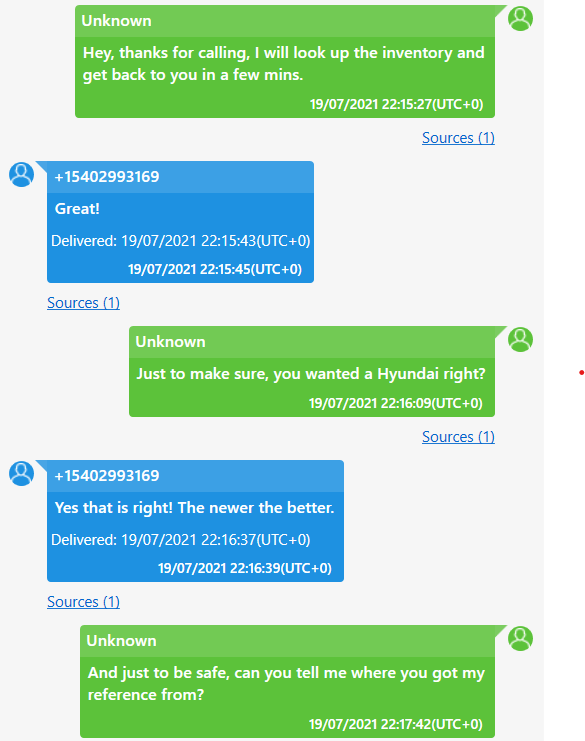
\includegraphics[width=\textwidth]{images/ss1.png}
        \caption{}
    \end{subfigure}
    \hspace{2 pt}
    \begin{subfigure}[b]{0.3\textwidth}
        \centering
        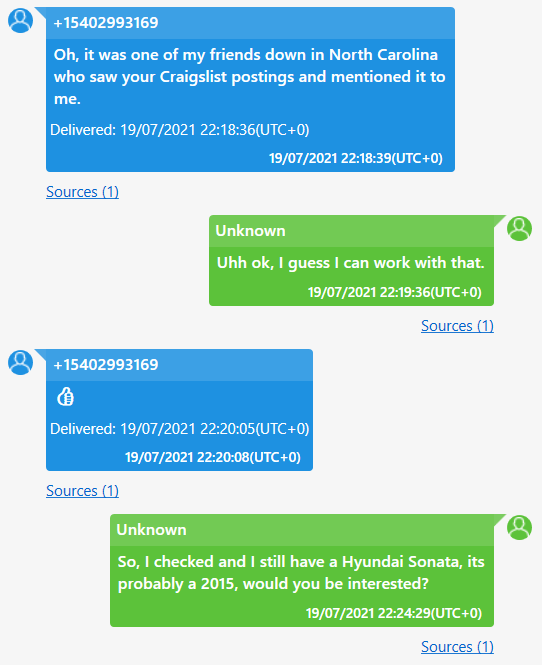
\includegraphics[width=\textwidth]{images/ss2.png}
        \caption{}
    \end{subfigure}
    \hspace{2 pt}
    \begin{subfigure}[b]{0.3\textwidth}
        \centering
        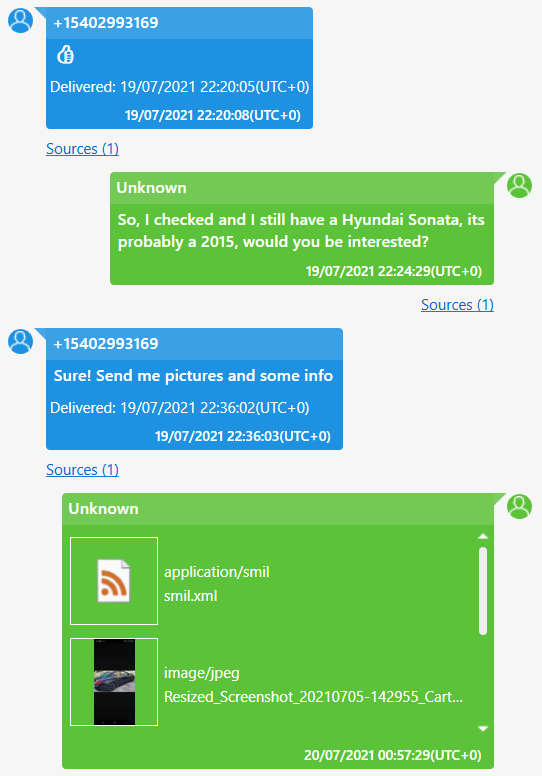
\includegraphics[width=\textwidth]{images/ss3.png}
        \caption{}
    \end{subfigure}
    \begin{subfigure}[b]{0.3\textwidth}
        \centering
        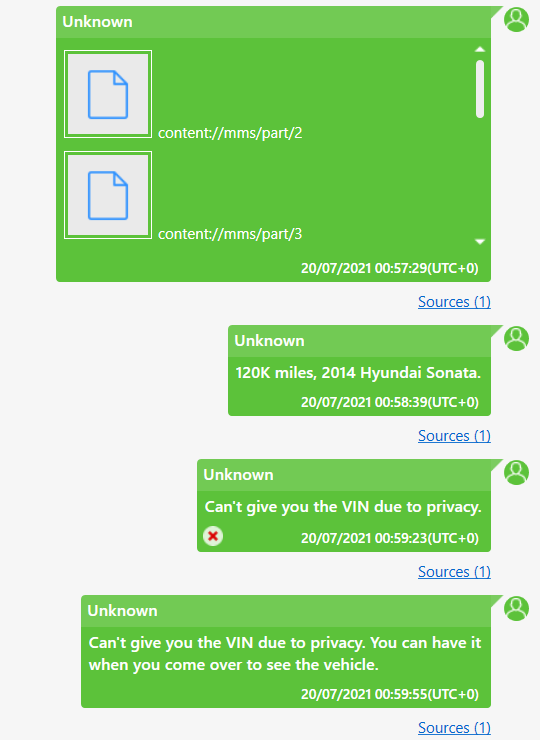
\includegraphics[width=\textwidth]{images/ss4.png}
        \caption{}
    \end{subfigure}
    \hspace{2 pt}
    \begin{subfigure}[b]{0.3\textwidth}
        \centering
        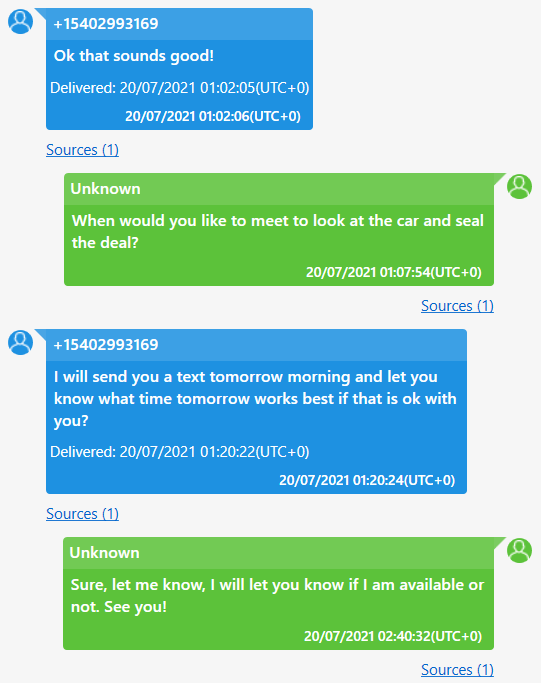
\includegraphics[width=\textwidth]{images/ss5.png}
        \caption{}
    \end{subfigure}
    \hspace{2 pt}
    \begin{subfigure}[b]{0.3\textwidth}
        \centering
        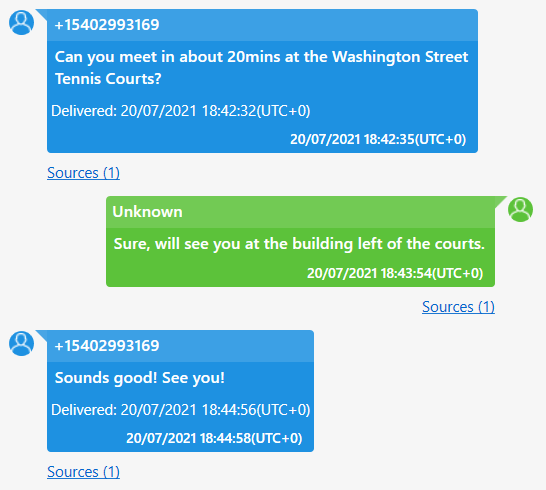
\includegraphics[width=\textwidth]{images/ss6-meeting.png}
        \caption{}
    \label{fig:meeting}
    \end{subfigure}
    \caption{Screenshots of the messages exchanged with \texttt{+15402993169}.}
    \label{fig:messages}
\end{figure}

You can see the pictures of the car he sent during the conversation with \texttt{+15402993169} in Figure \ref{fig:cars}.
The paths of the pictures are the following:
\begin{itemize}
    \item \texttt{Dump/data/user\_de/0/com.android.providers.telephony/app\_parts/\\PART\_1626742644543\_Resized\_Screenshot\_20210705-142955\_Cartomizer.jpeg}
    \item \texttt{Dump/data/user\_de/0/com.android.providers.telephony/app\_parts/\\PART\_1626742644555\_Resized\_20210703\_192751.jpeg}
    \item \texttt{Dump/data/user\_de/0/com.android.providers.telephony/app\_parts/\\PART\_1626742644568\_Resized\_20210703\_192806.jpeg}
\end{itemize}

\begin{figure}[!ht]
    \centering
    \begin{subfigure}[b]{0.3\textwidth}
        \centering
        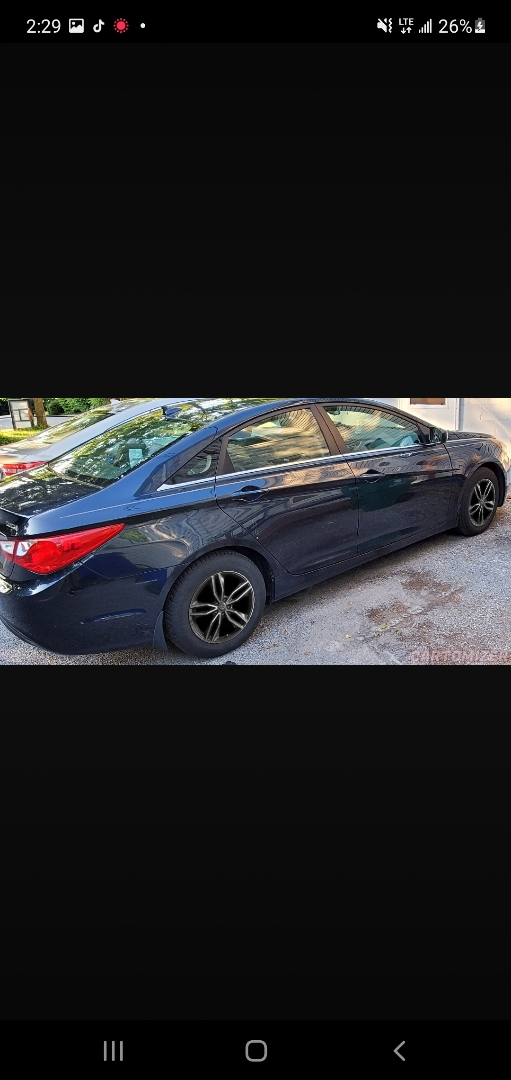
\includegraphics[width=\textwidth]{images/car1.png}
        \caption{}
    \end{subfigure}
    \hspace{2 pt}
    \begin{subfigure}[b]{0.3\textwidth}
        \centering
        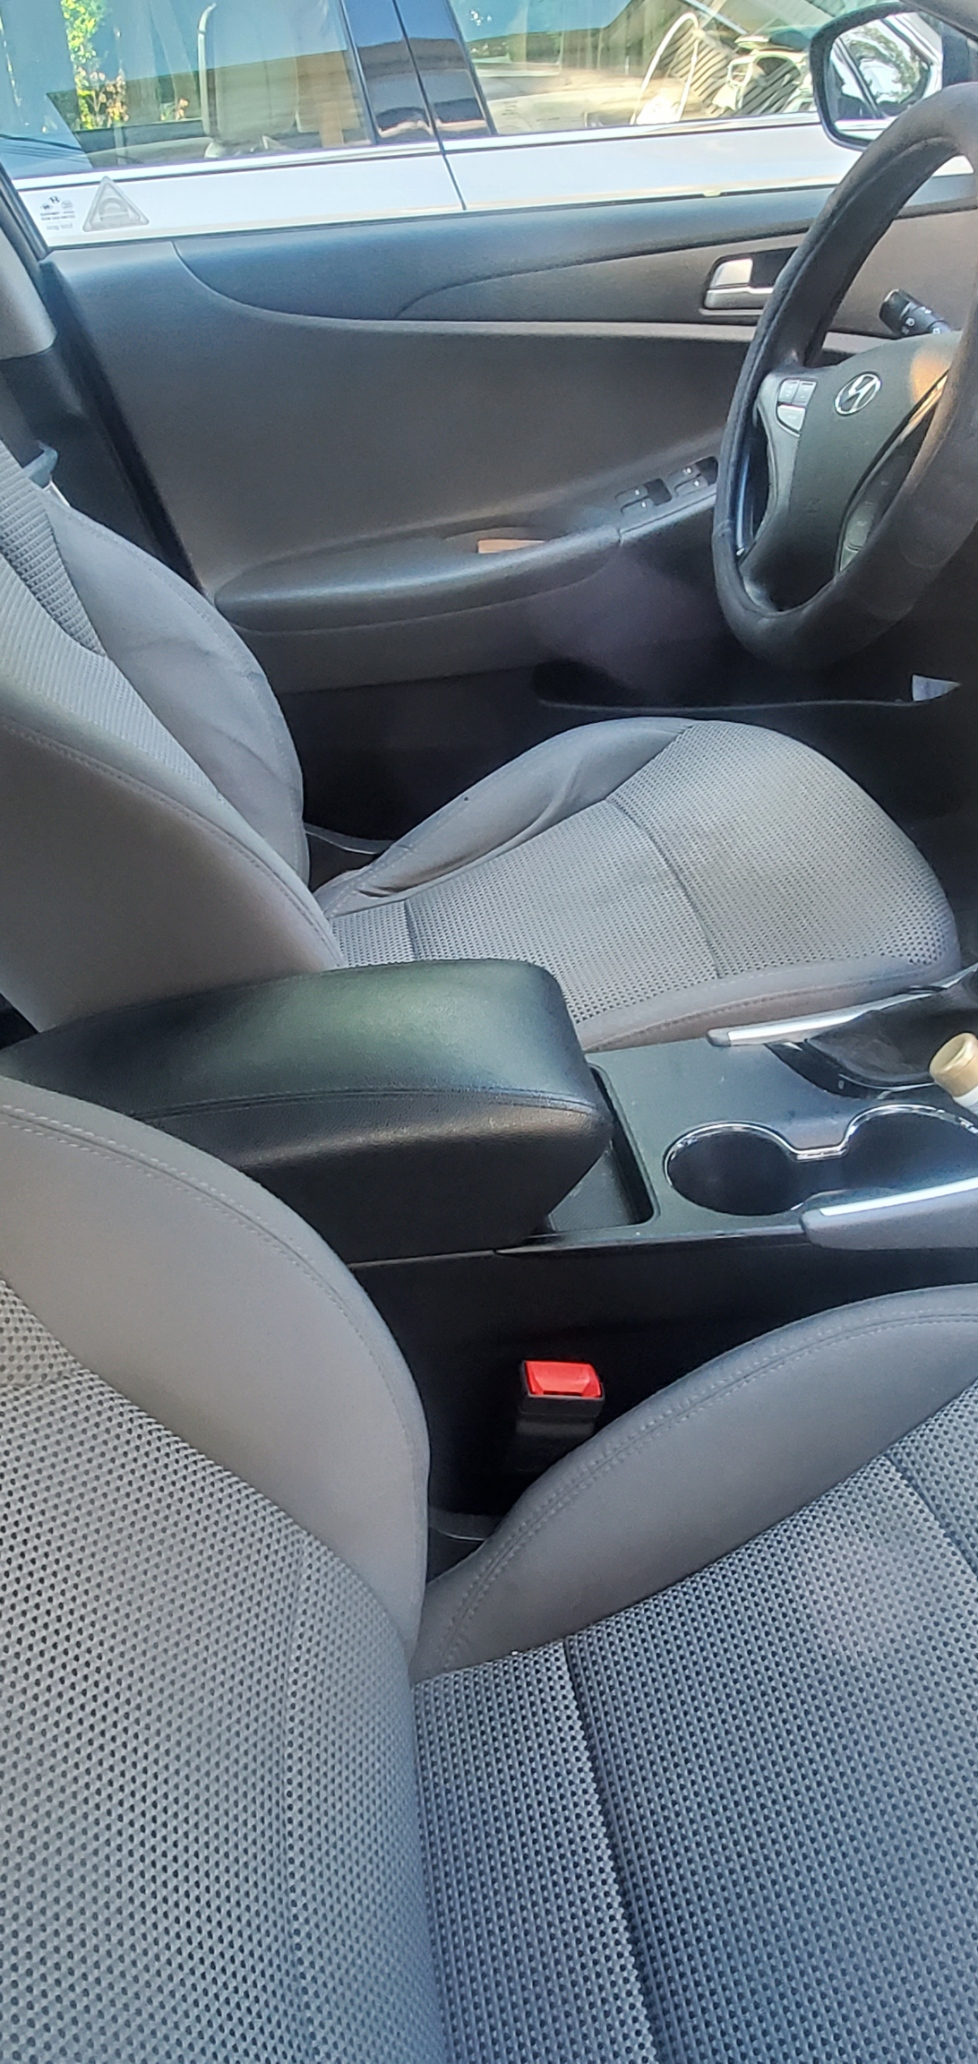
\includegraphics[width=\textwidth]{images/car2.png}
        \caption{}
    \end{subfigure} \\
    \vspace{3 pt}
    \begin{subfigure}[b]{0.6\textwidth}
        \centering
        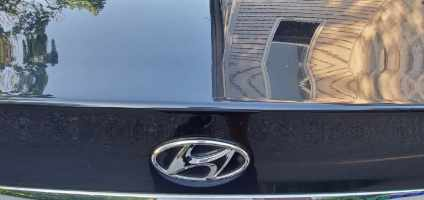
\includegraphics[width=\textwidth]{images/car3.png}
        \caption{}
    \end{subfigure}
    \caption{Pictures of the car that Heisenberg was selling.}
    \label{fig:cars}
\end{figure}

Moreover, I found some other messages with a contact called Beth Dutton in Instagram, where there are death menaces from her. This indicates that Heisenberg was conducting sketchy business. 

You can see the messages in Figure \ref{fig:messages2} and the hash of the DB containing Instagram direct messages in the table \ref{table:hashes}.

\begin{figure}[!ht]
    \centering
    \begin{subfigure}[b]{0.3\textwidth}
        \centering
        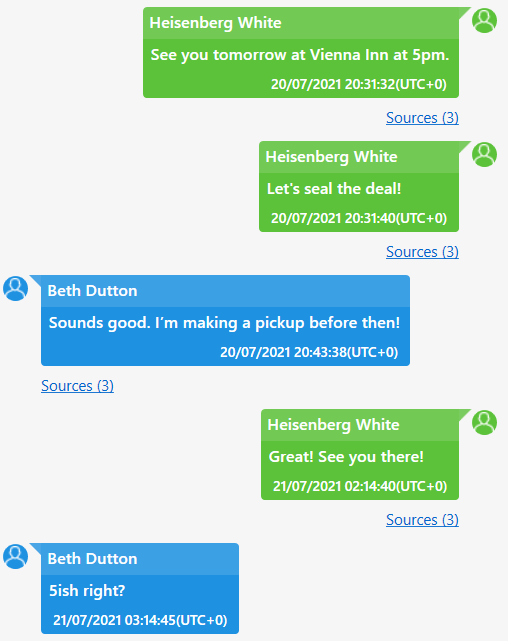
\includegraphics[width=\textwidth]{images/beth1.png}
        \caption{}
    \end{subfigure}
    \hspace{2 pt}
    \begin{subfigure}[b]{0.3\textwidth}
        \centering
        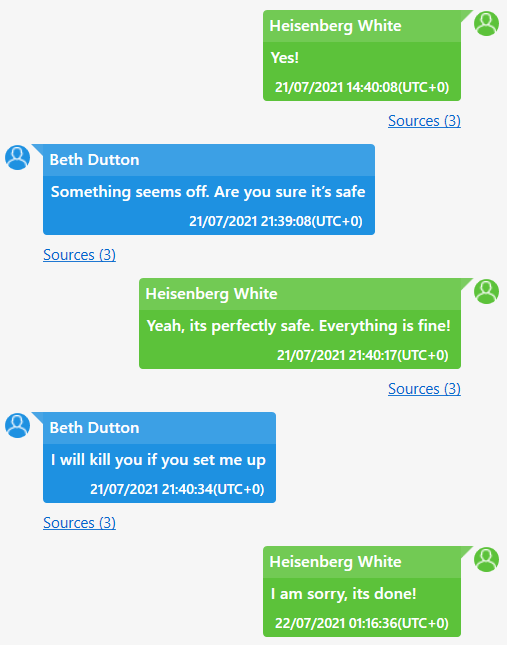
\includegraphics[width=\textwidth]{images/beth2.png}
        \caption{}
    \end{subfigure}
    \caption{Screenshots of the messages exchanged with Beth Dutton.}
    \label{fig:messages2}
\end{figure}

As I already mentioned, there are many pictures of cars in his smartphone, but they are related to the apps installed on the smartphone. So I looked for pictures with capture time in the DCMI folder: in this way we can suppose that the pictures were taken by Heisenberg. I found 10 pictures of cars in this way, which are shown in Figure \ref{fig:cars2}. All the pictures are in the folder \texttt{Dump/data/media/0/DCIM} and you can check their names and hashes in the table \ref{table:hashes-cars}.

\begin{figure}[!ht]
    \centering
    \begin{subfigure}[b]{0.4\textwidth}
        \centering
        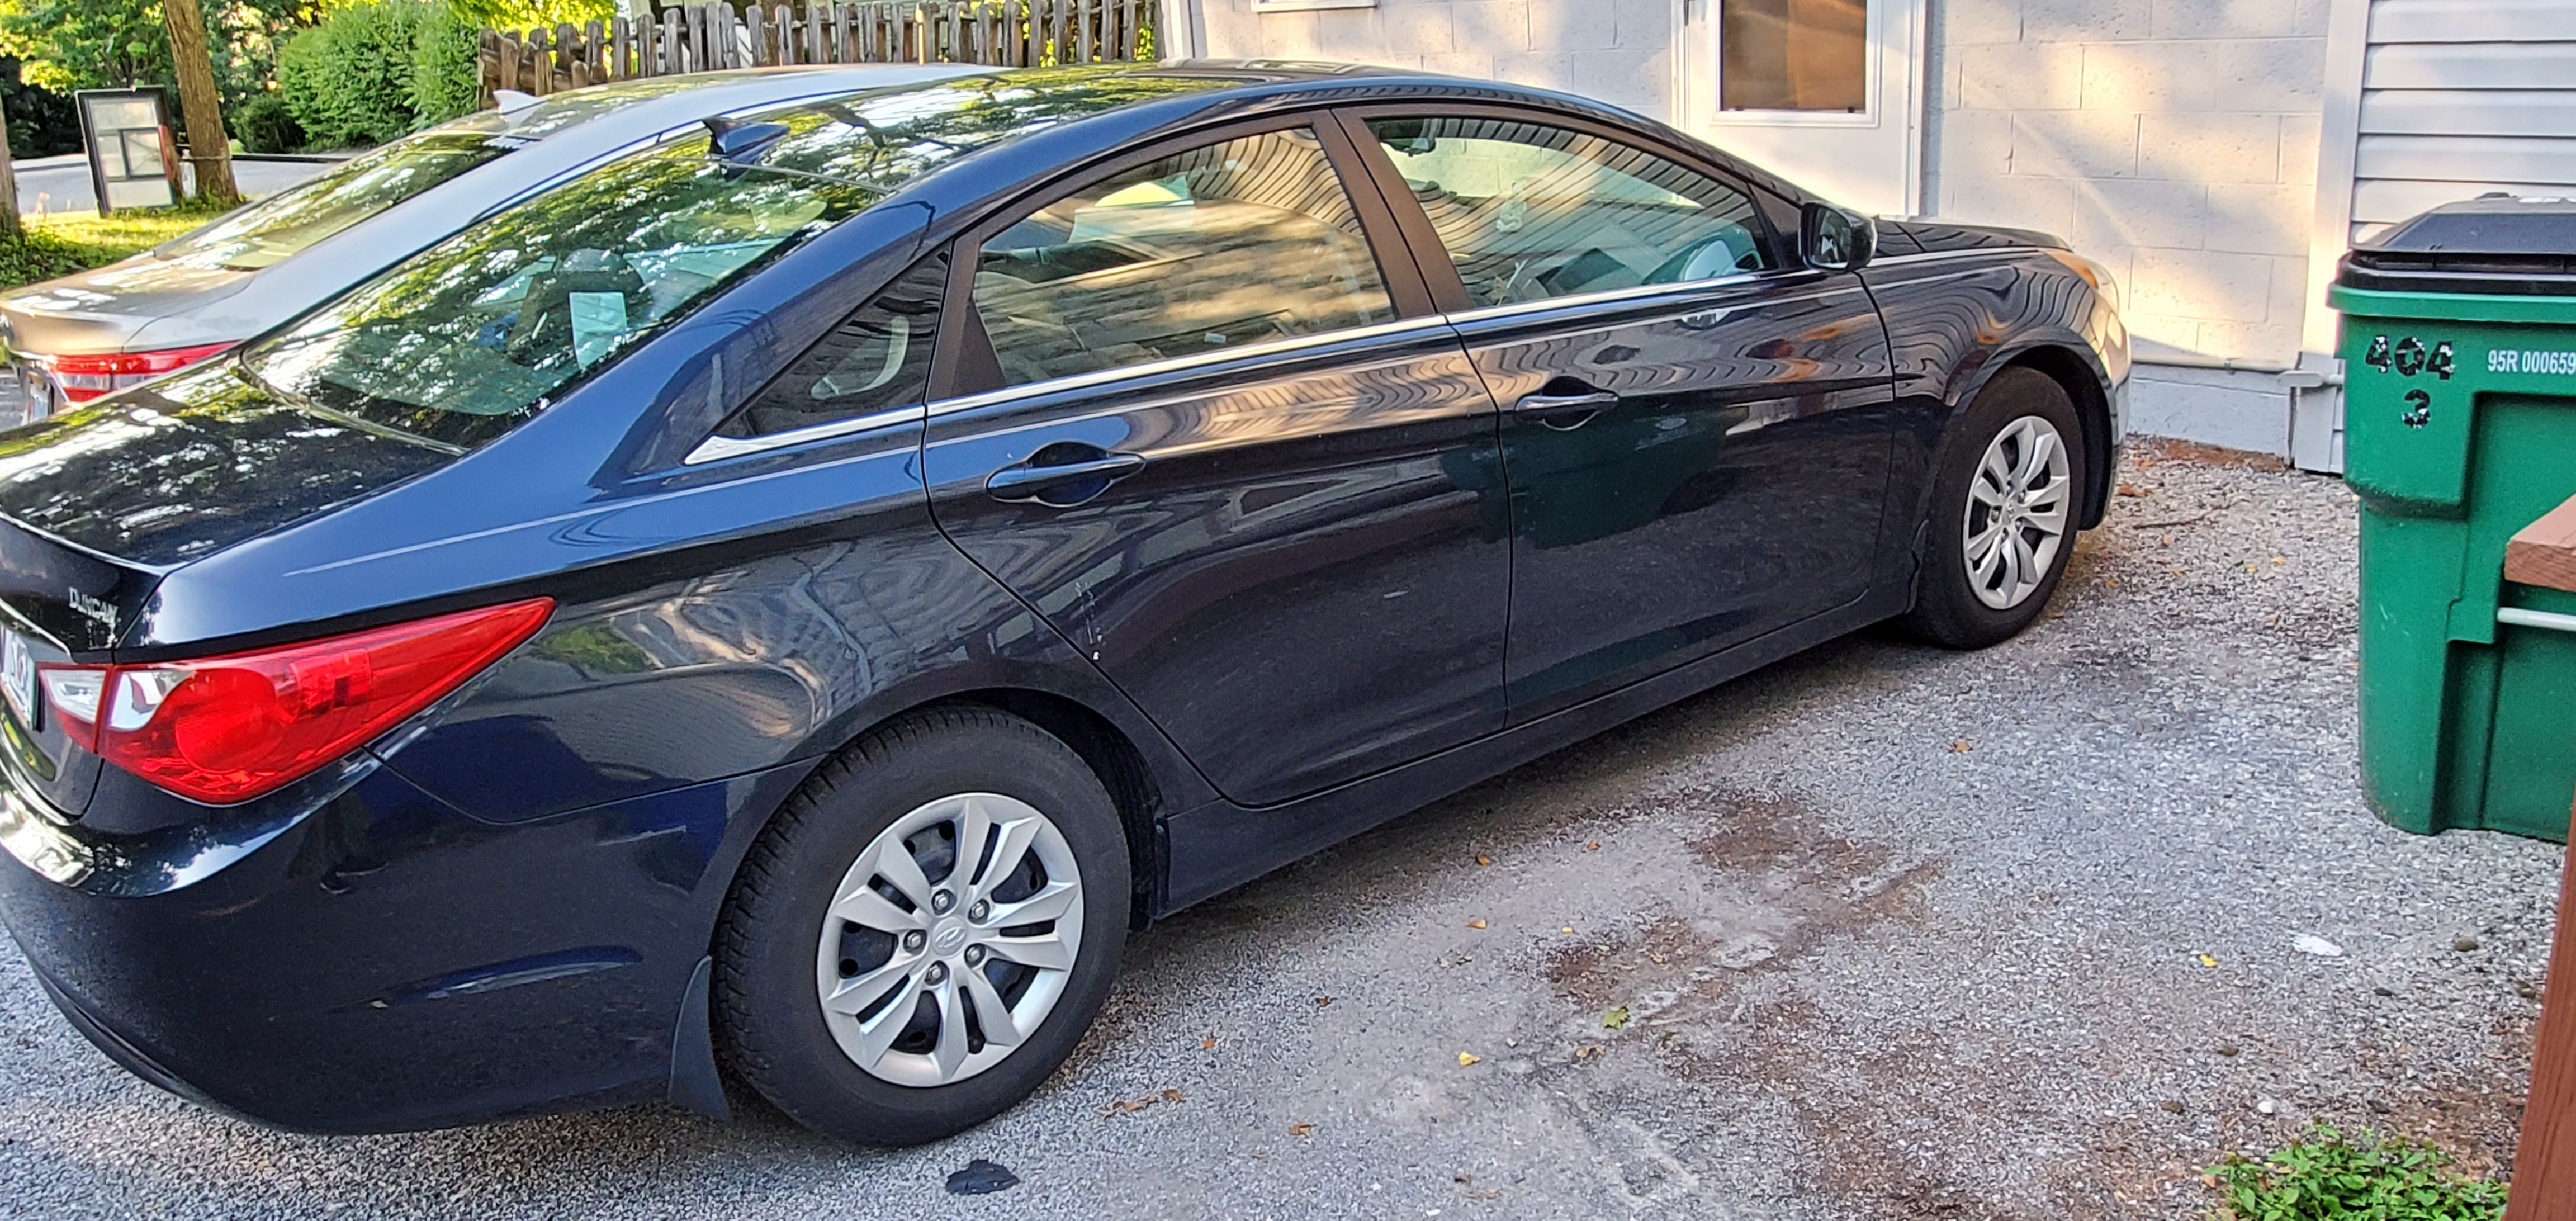
\includegraphics[width=\textwidth]{images/car_photos/20210703_192737.jpg} %1
        \caption{}
    \end{subfigure}
    \hspace{2 pt}
    \begin{subfigure}[b]{0.4\textwidth}
        \centering
        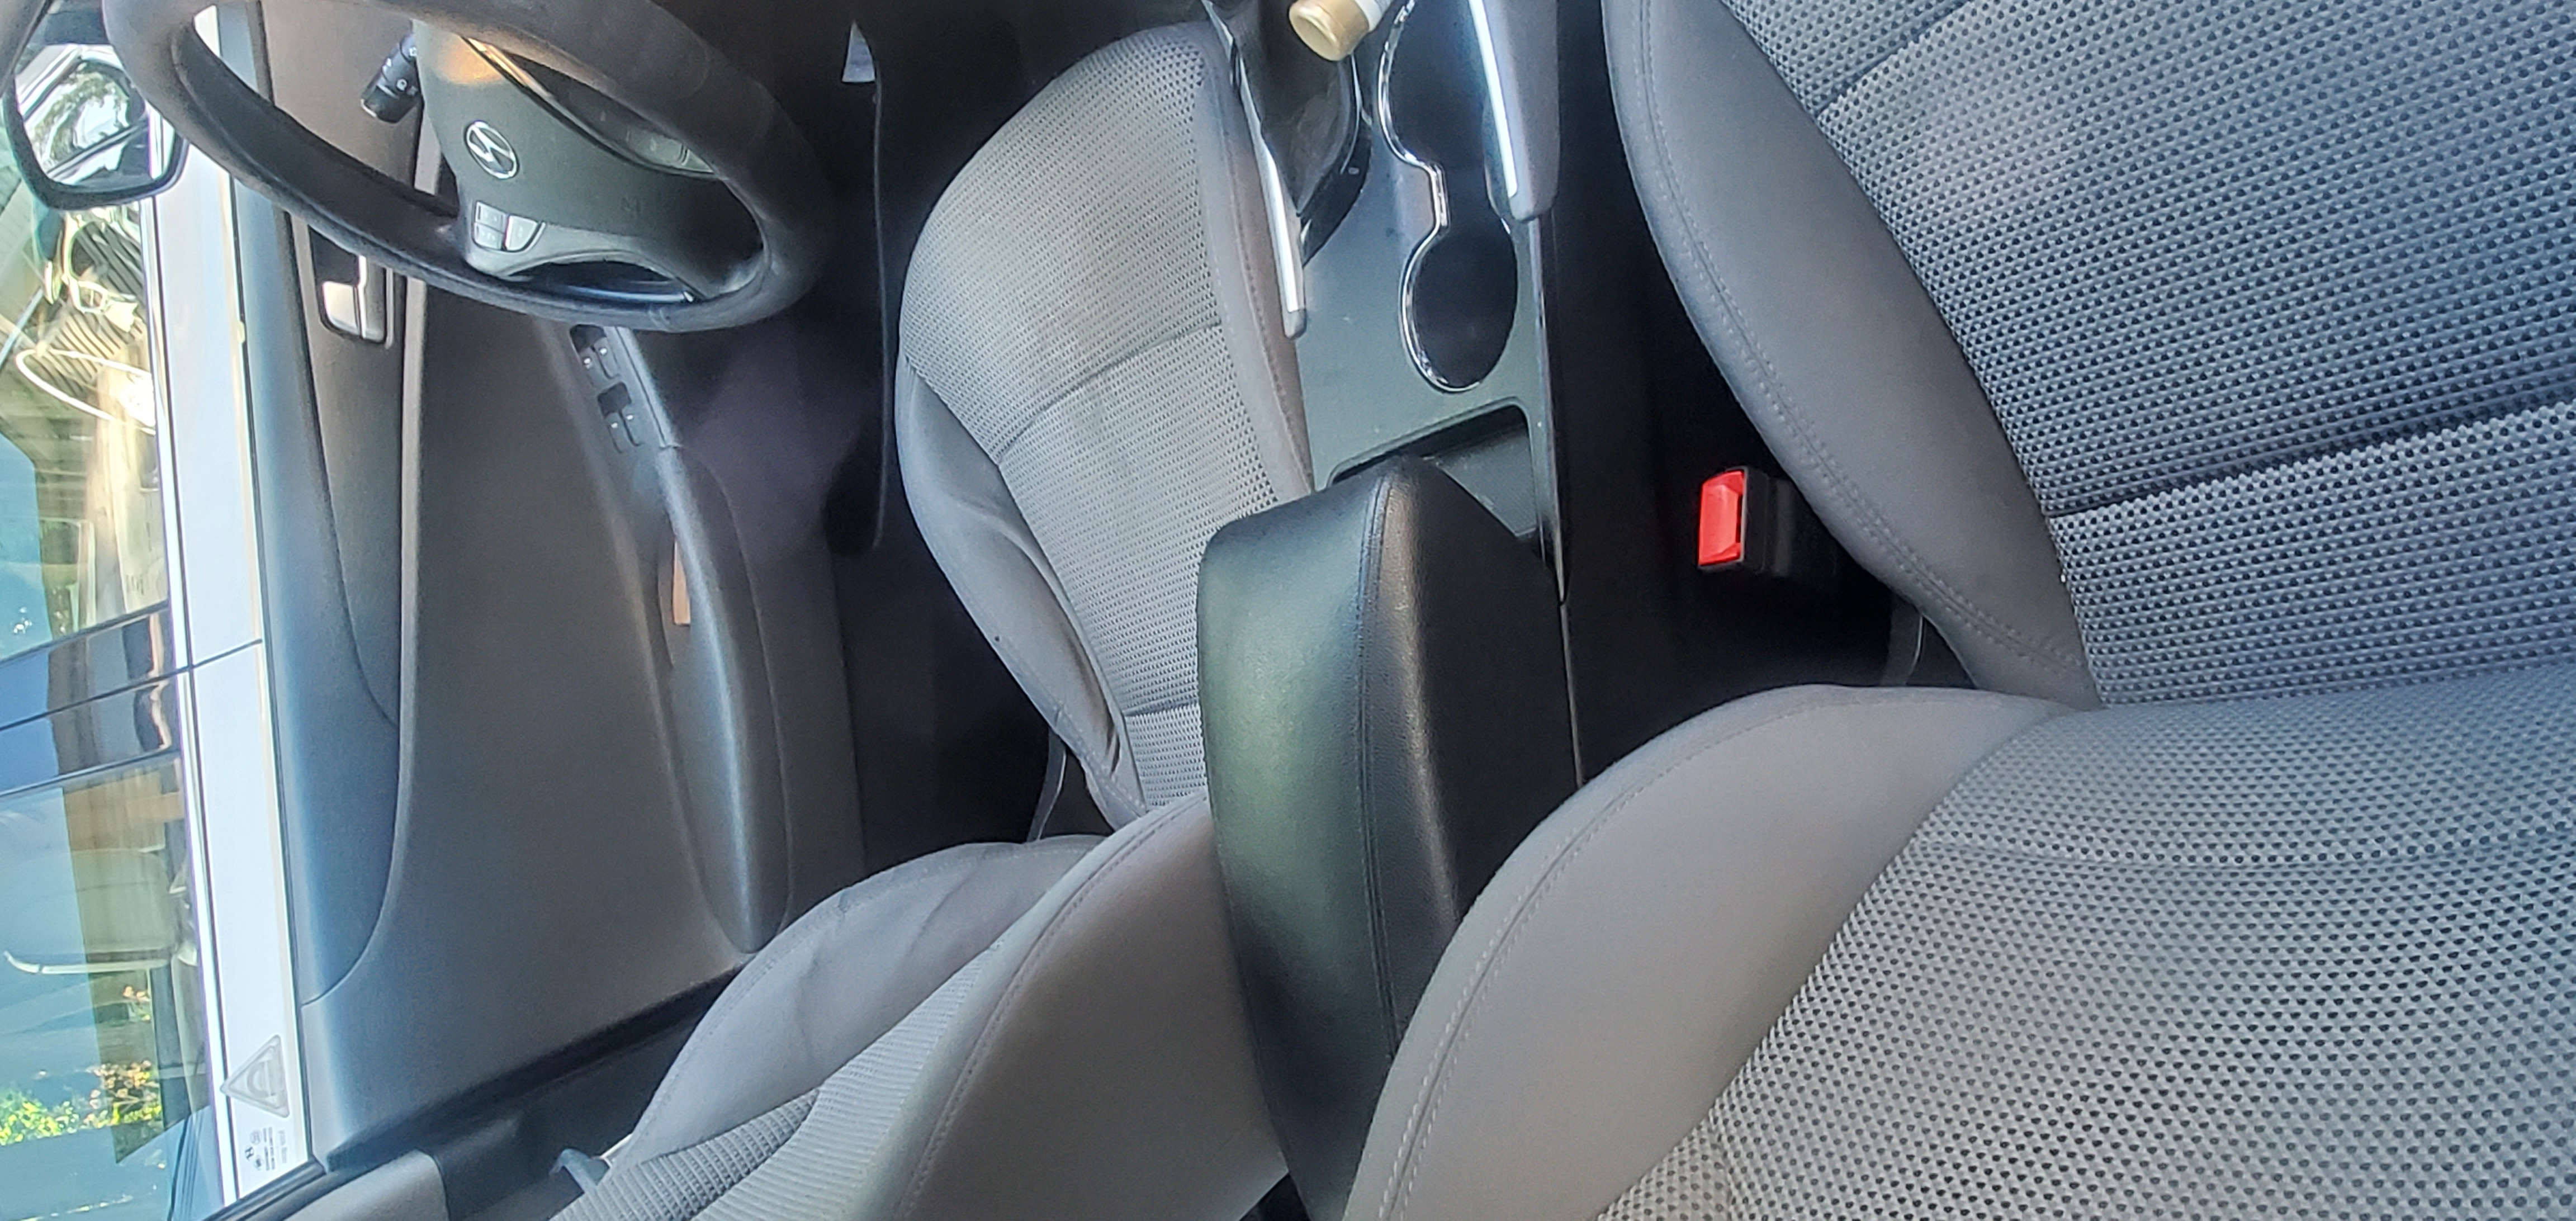
\includegraphics[width=\textwidth]{images/car_photos/20210703_192751.jpg} %2
        \caption{}
    \end{subfigure}
    \begin{subfigure}[b]{0.4\textwidth}
        \centering
        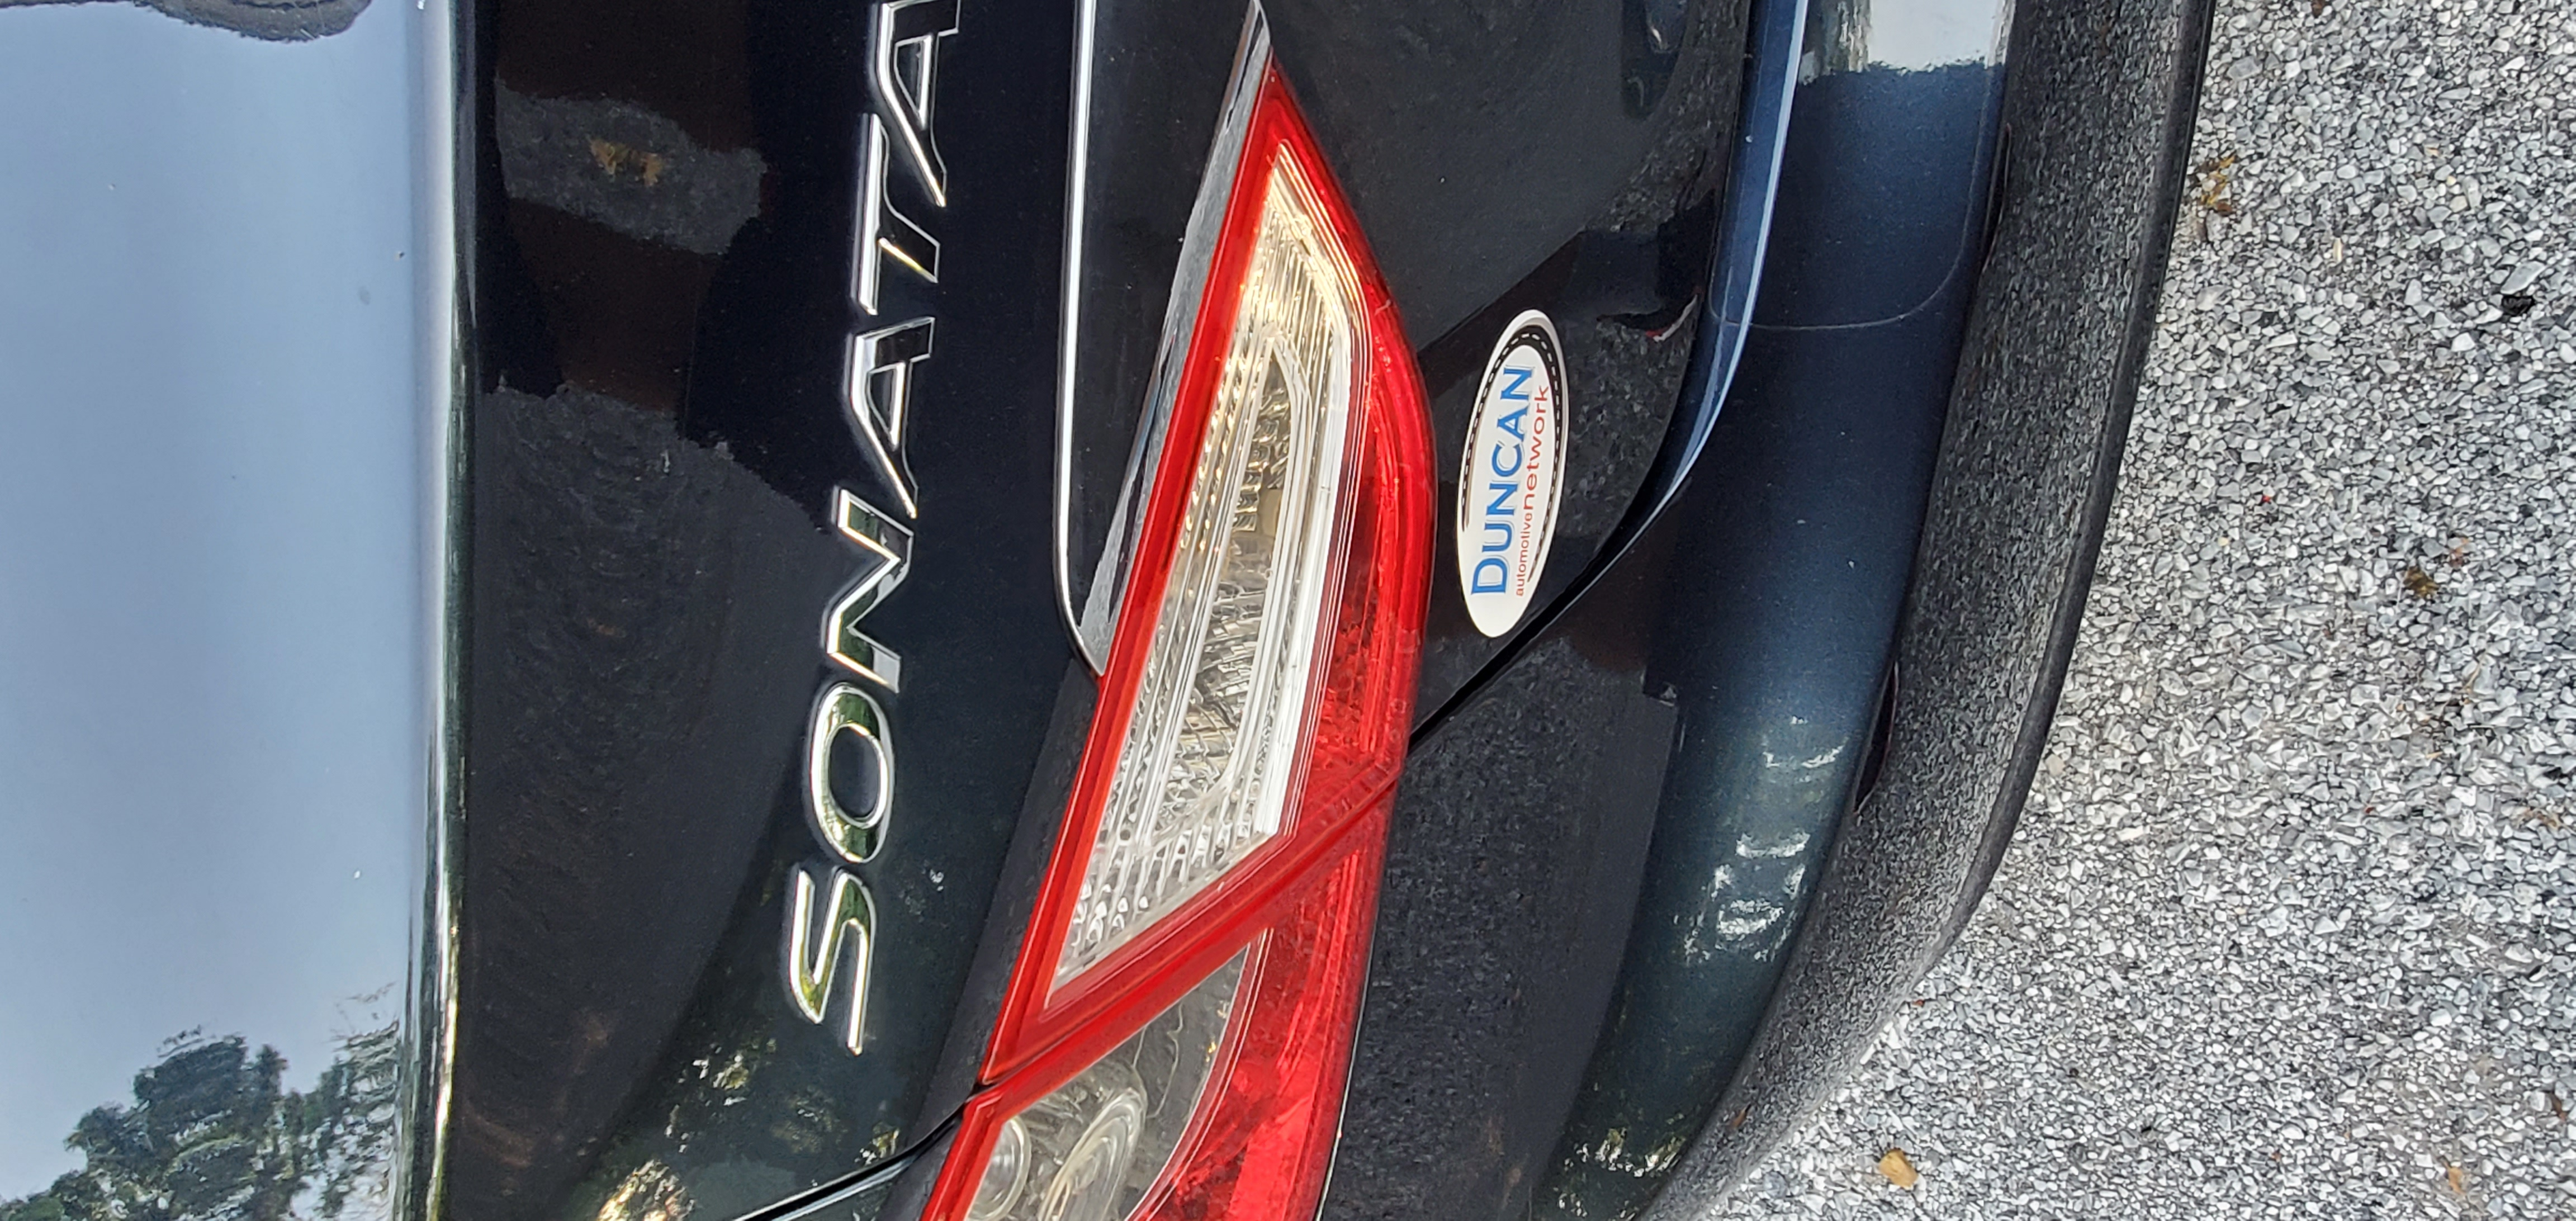
\includegraphics[width=\textwidth]{images/car_photos/20210703_192759.jpg} %3
        \caption{}
    \end{subfigure}
    \hspace{2 pt}
    \begin{subfigure}[b]{0.4\textwidth}
        \centering
        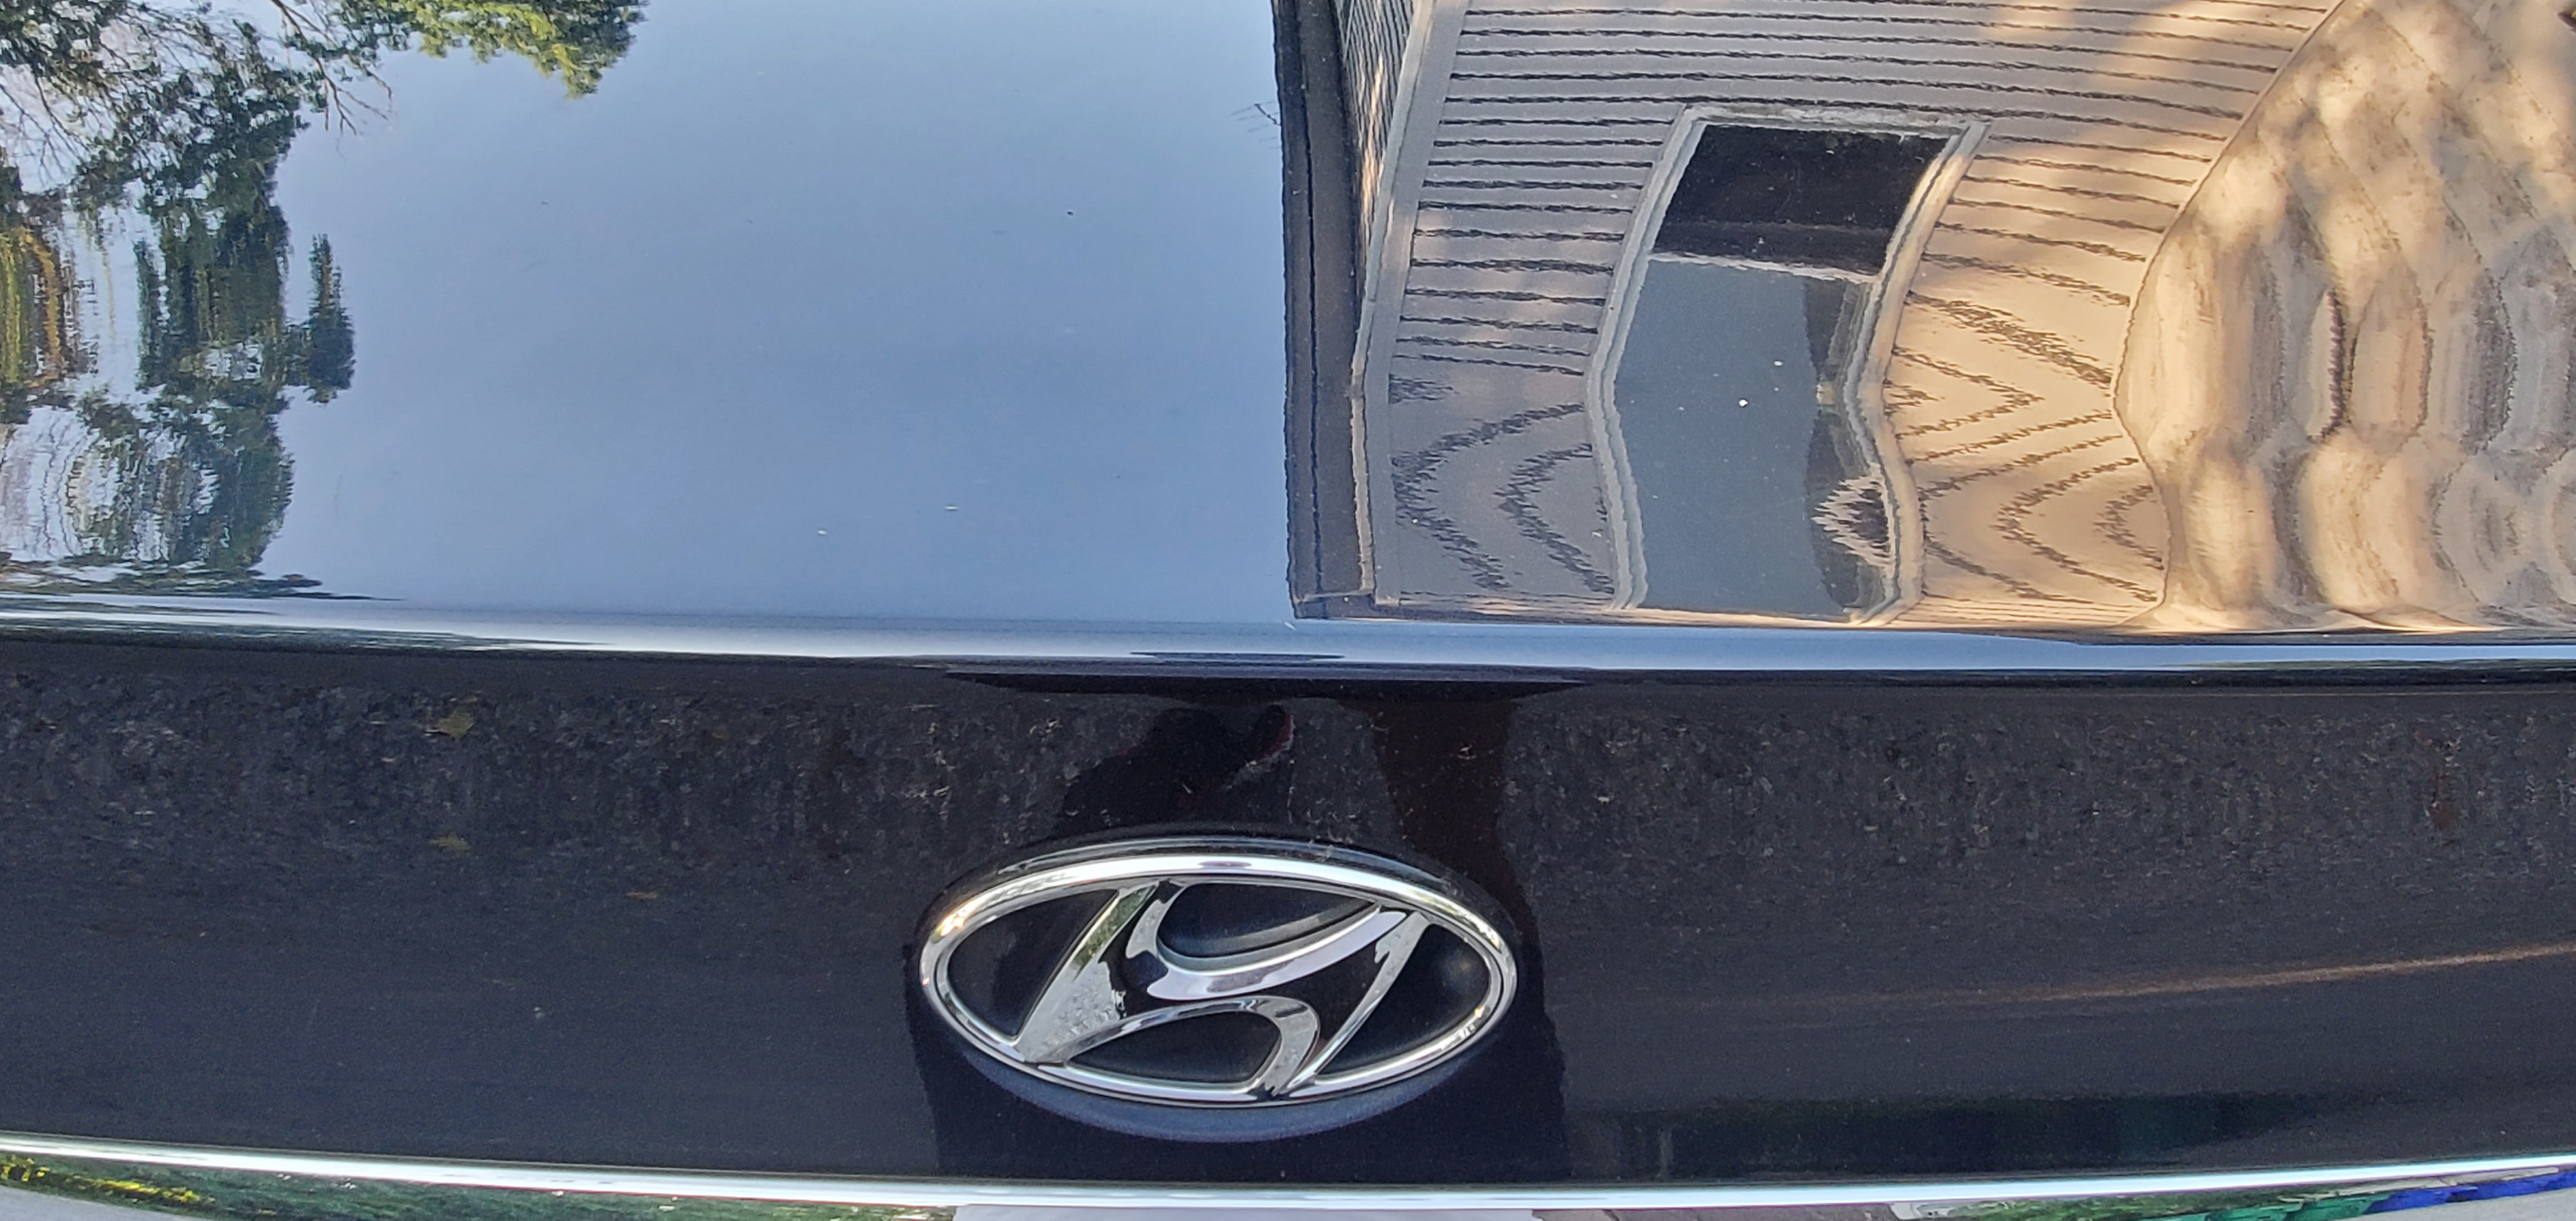
\includegraphics[width=\textwidth]{images/car_photos/20210703_192806.jpg} %4
        \caption{}
    \end{subfigure}
    \begin{subfigure}[b]{0.4\textwidth}
        \centering
        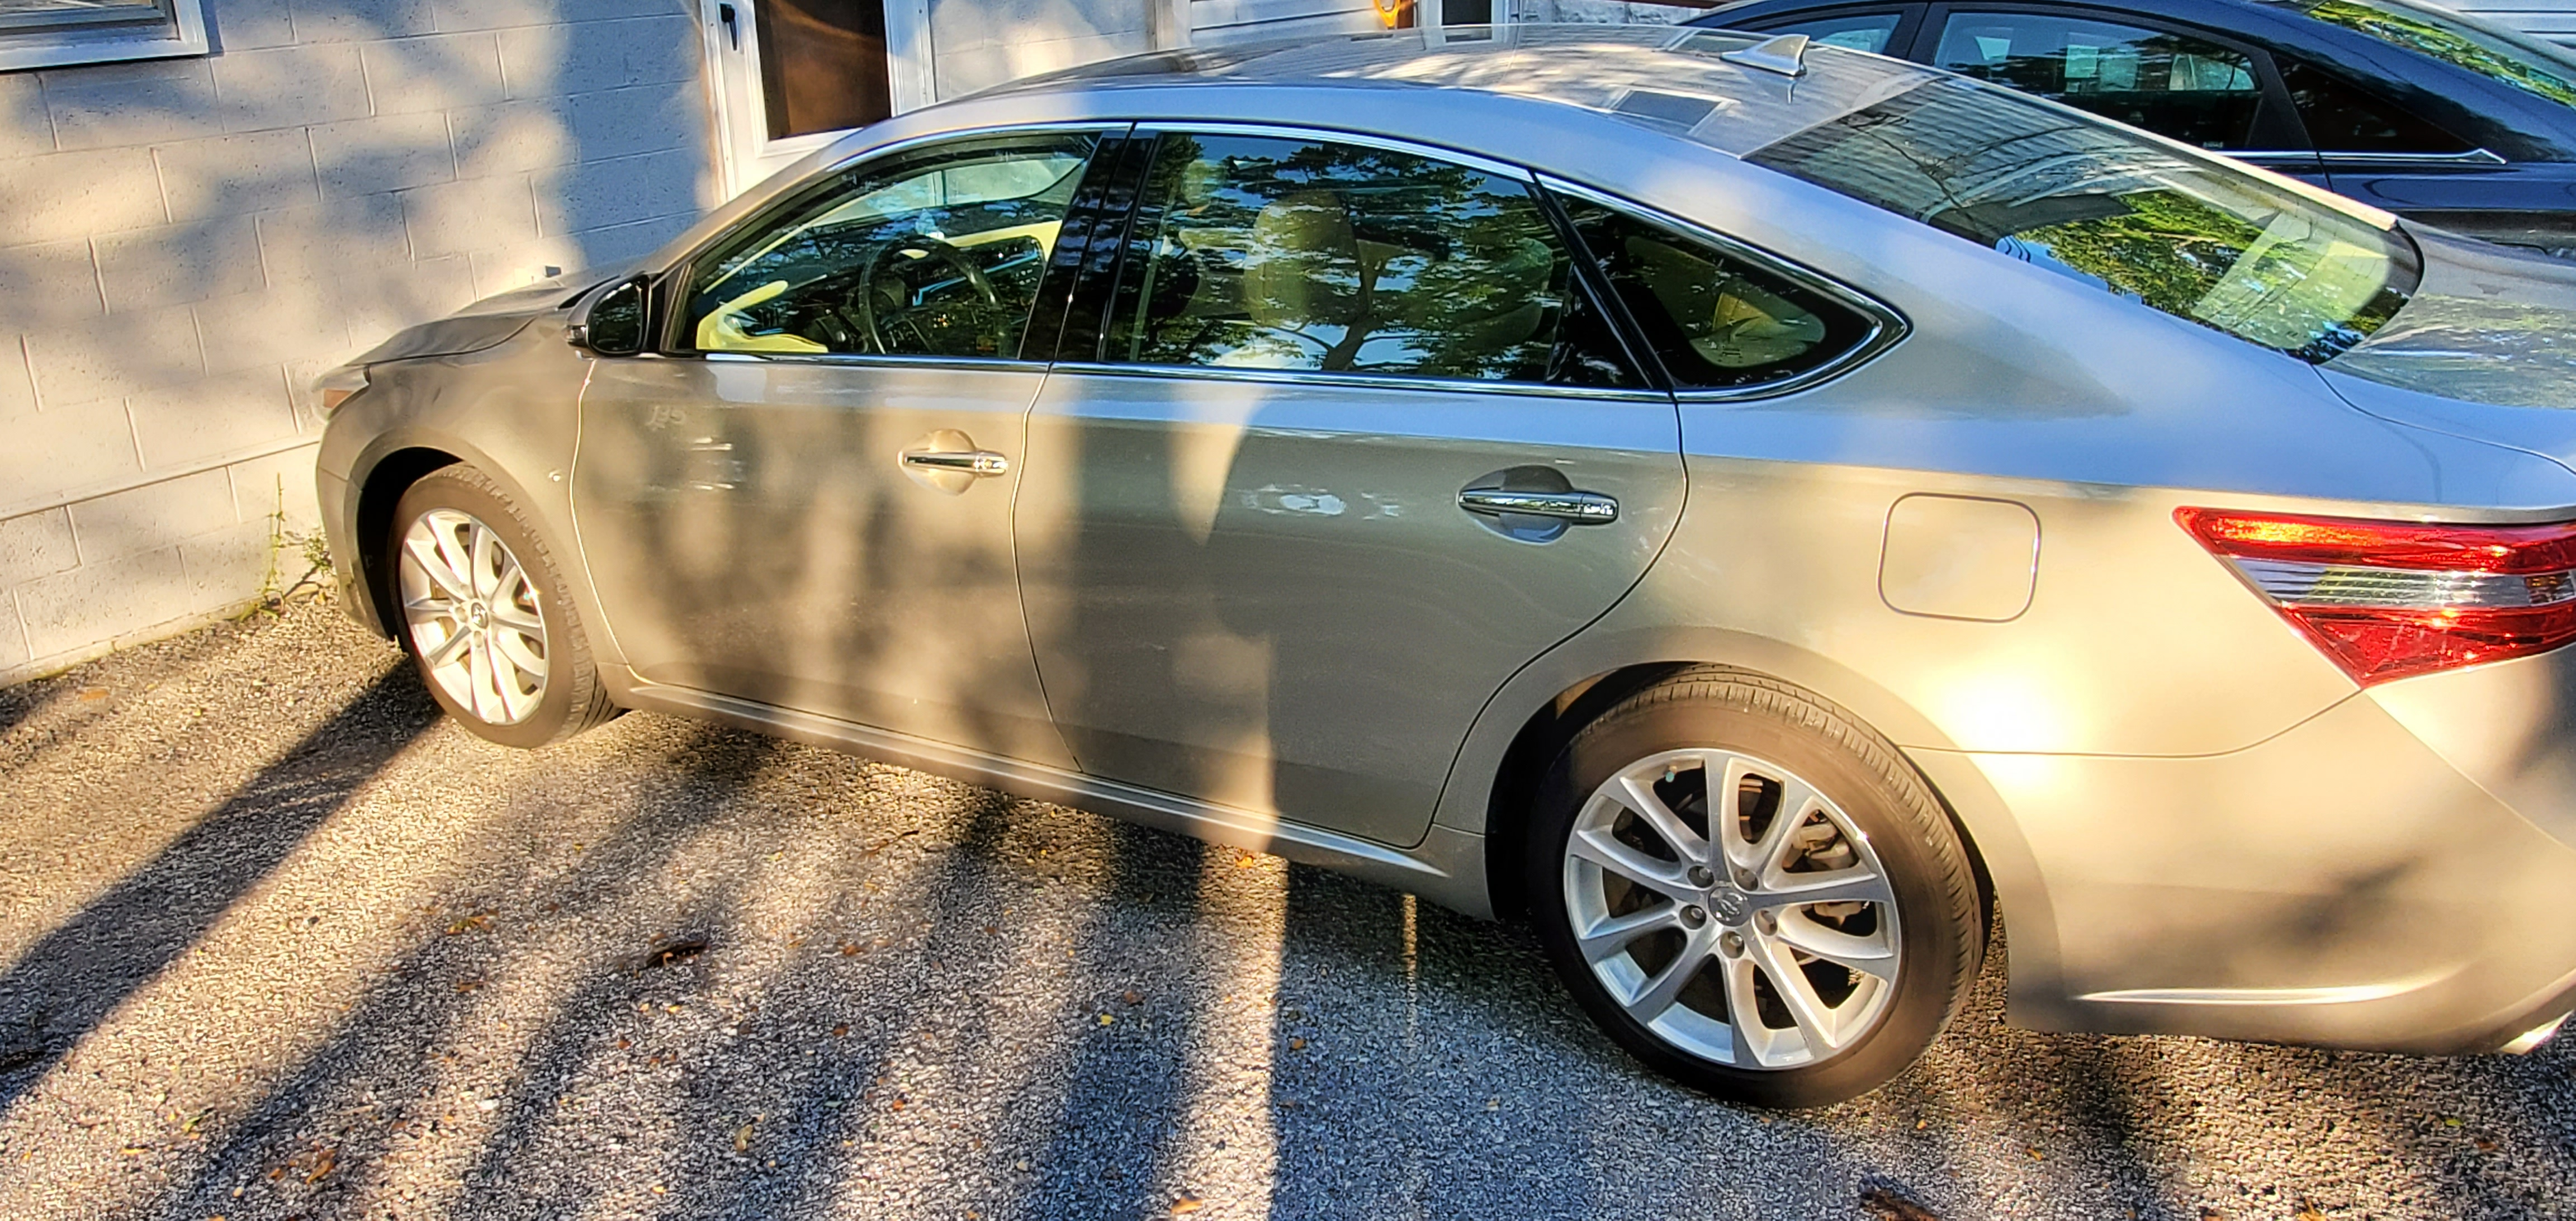
\includegraphics[width=\textwidth]{images/car_photos/20210703_192822.jpg} %5
        \caption{}
    \end{subfigure}
    \hspace{2 pt}
    \begin{subfigure}[b]{0.4\textwidth}
        \centering
        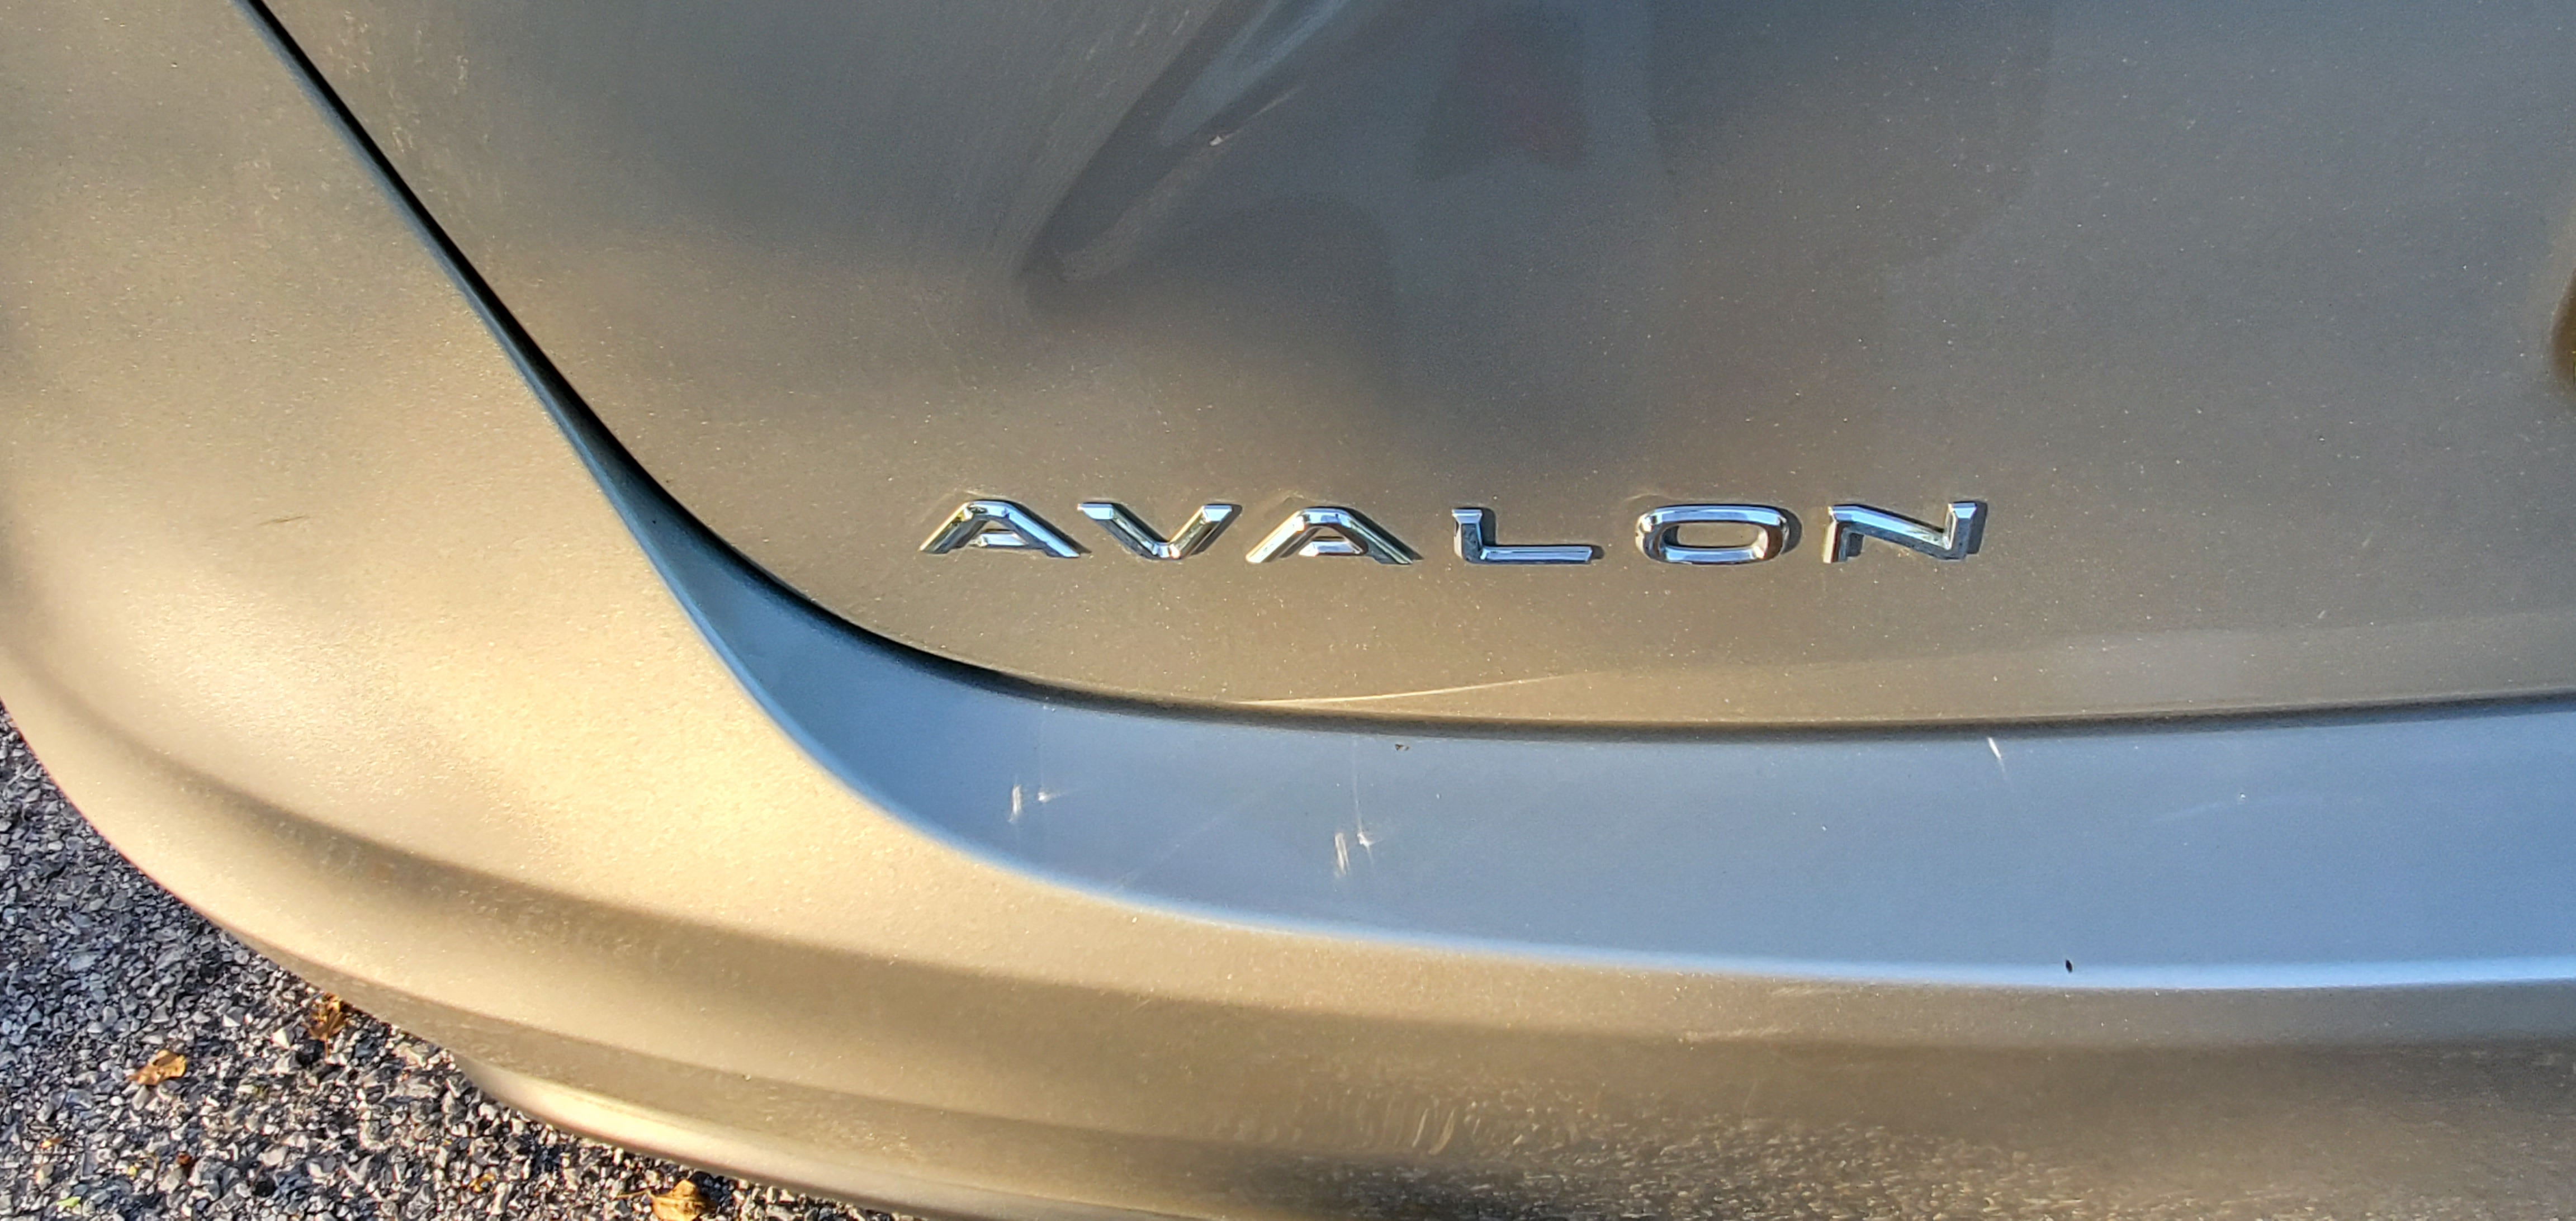
\includegraphics[width=\textwidth]{images/car_photos/20210703_192830.jpg} %6
        \caption{}
    \end{subfigure}
    \begin{subfigure}[b]{0.4\textwidth}
        \centering
        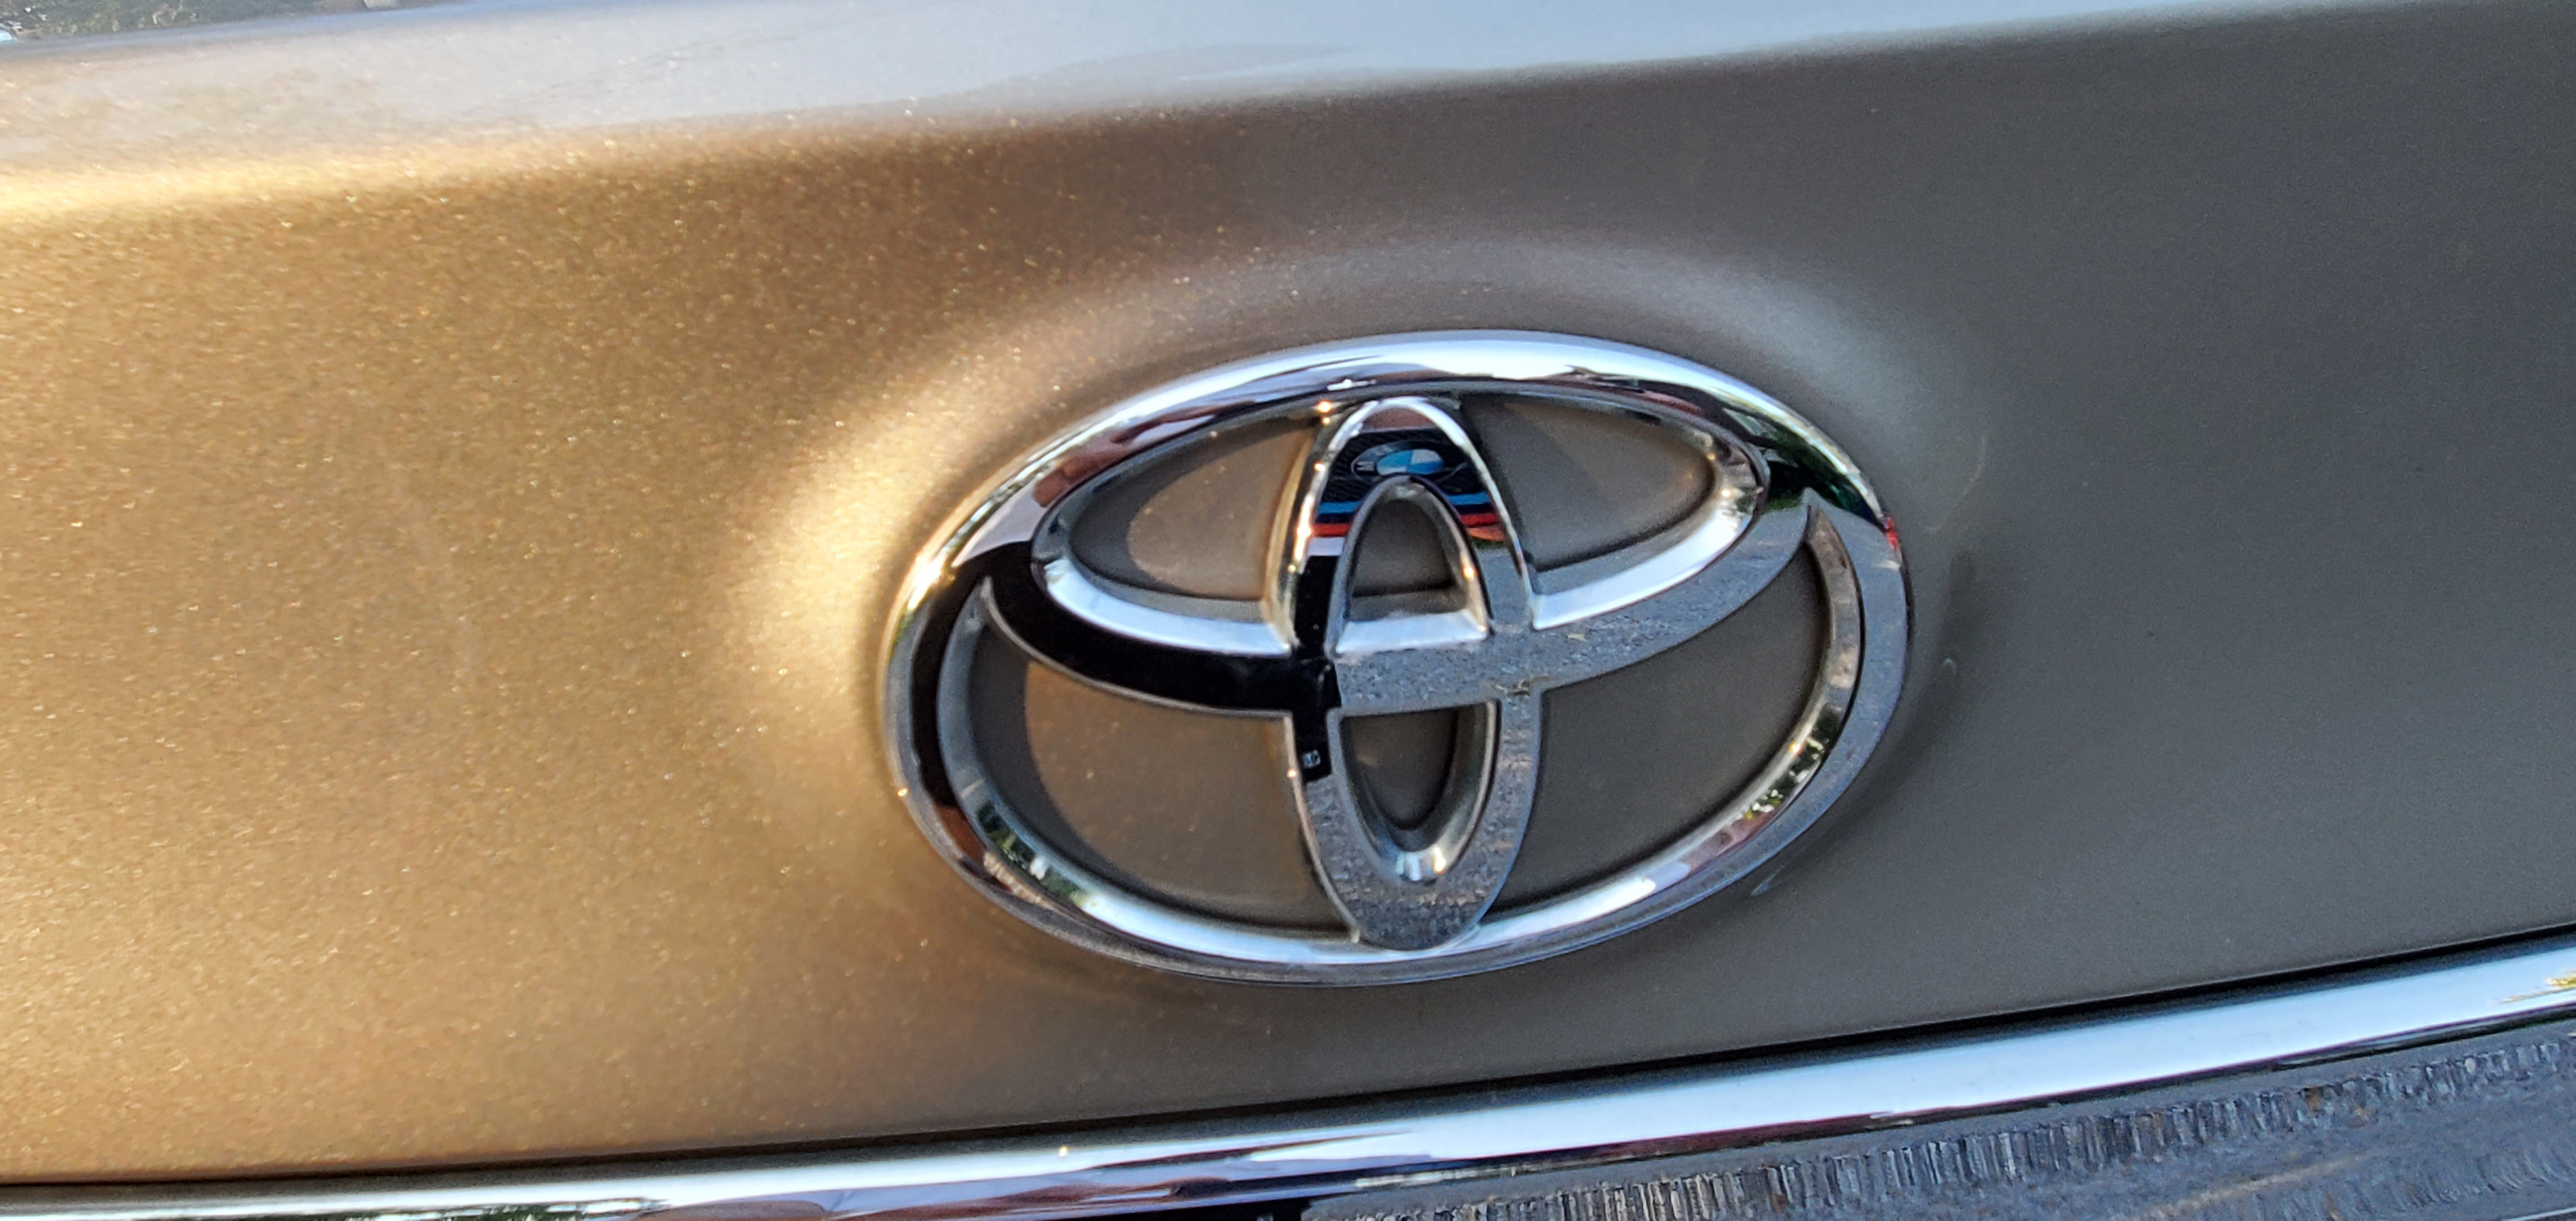
\includegraphics[width=\textwidth]{images/car_photos/20210703_192836.jpg} %7
        \caption{}
    \end{subfigure}
    \hspace{2 pt}
    \begin{subfigure}[b]{0.4\textwidth}
        \centering
        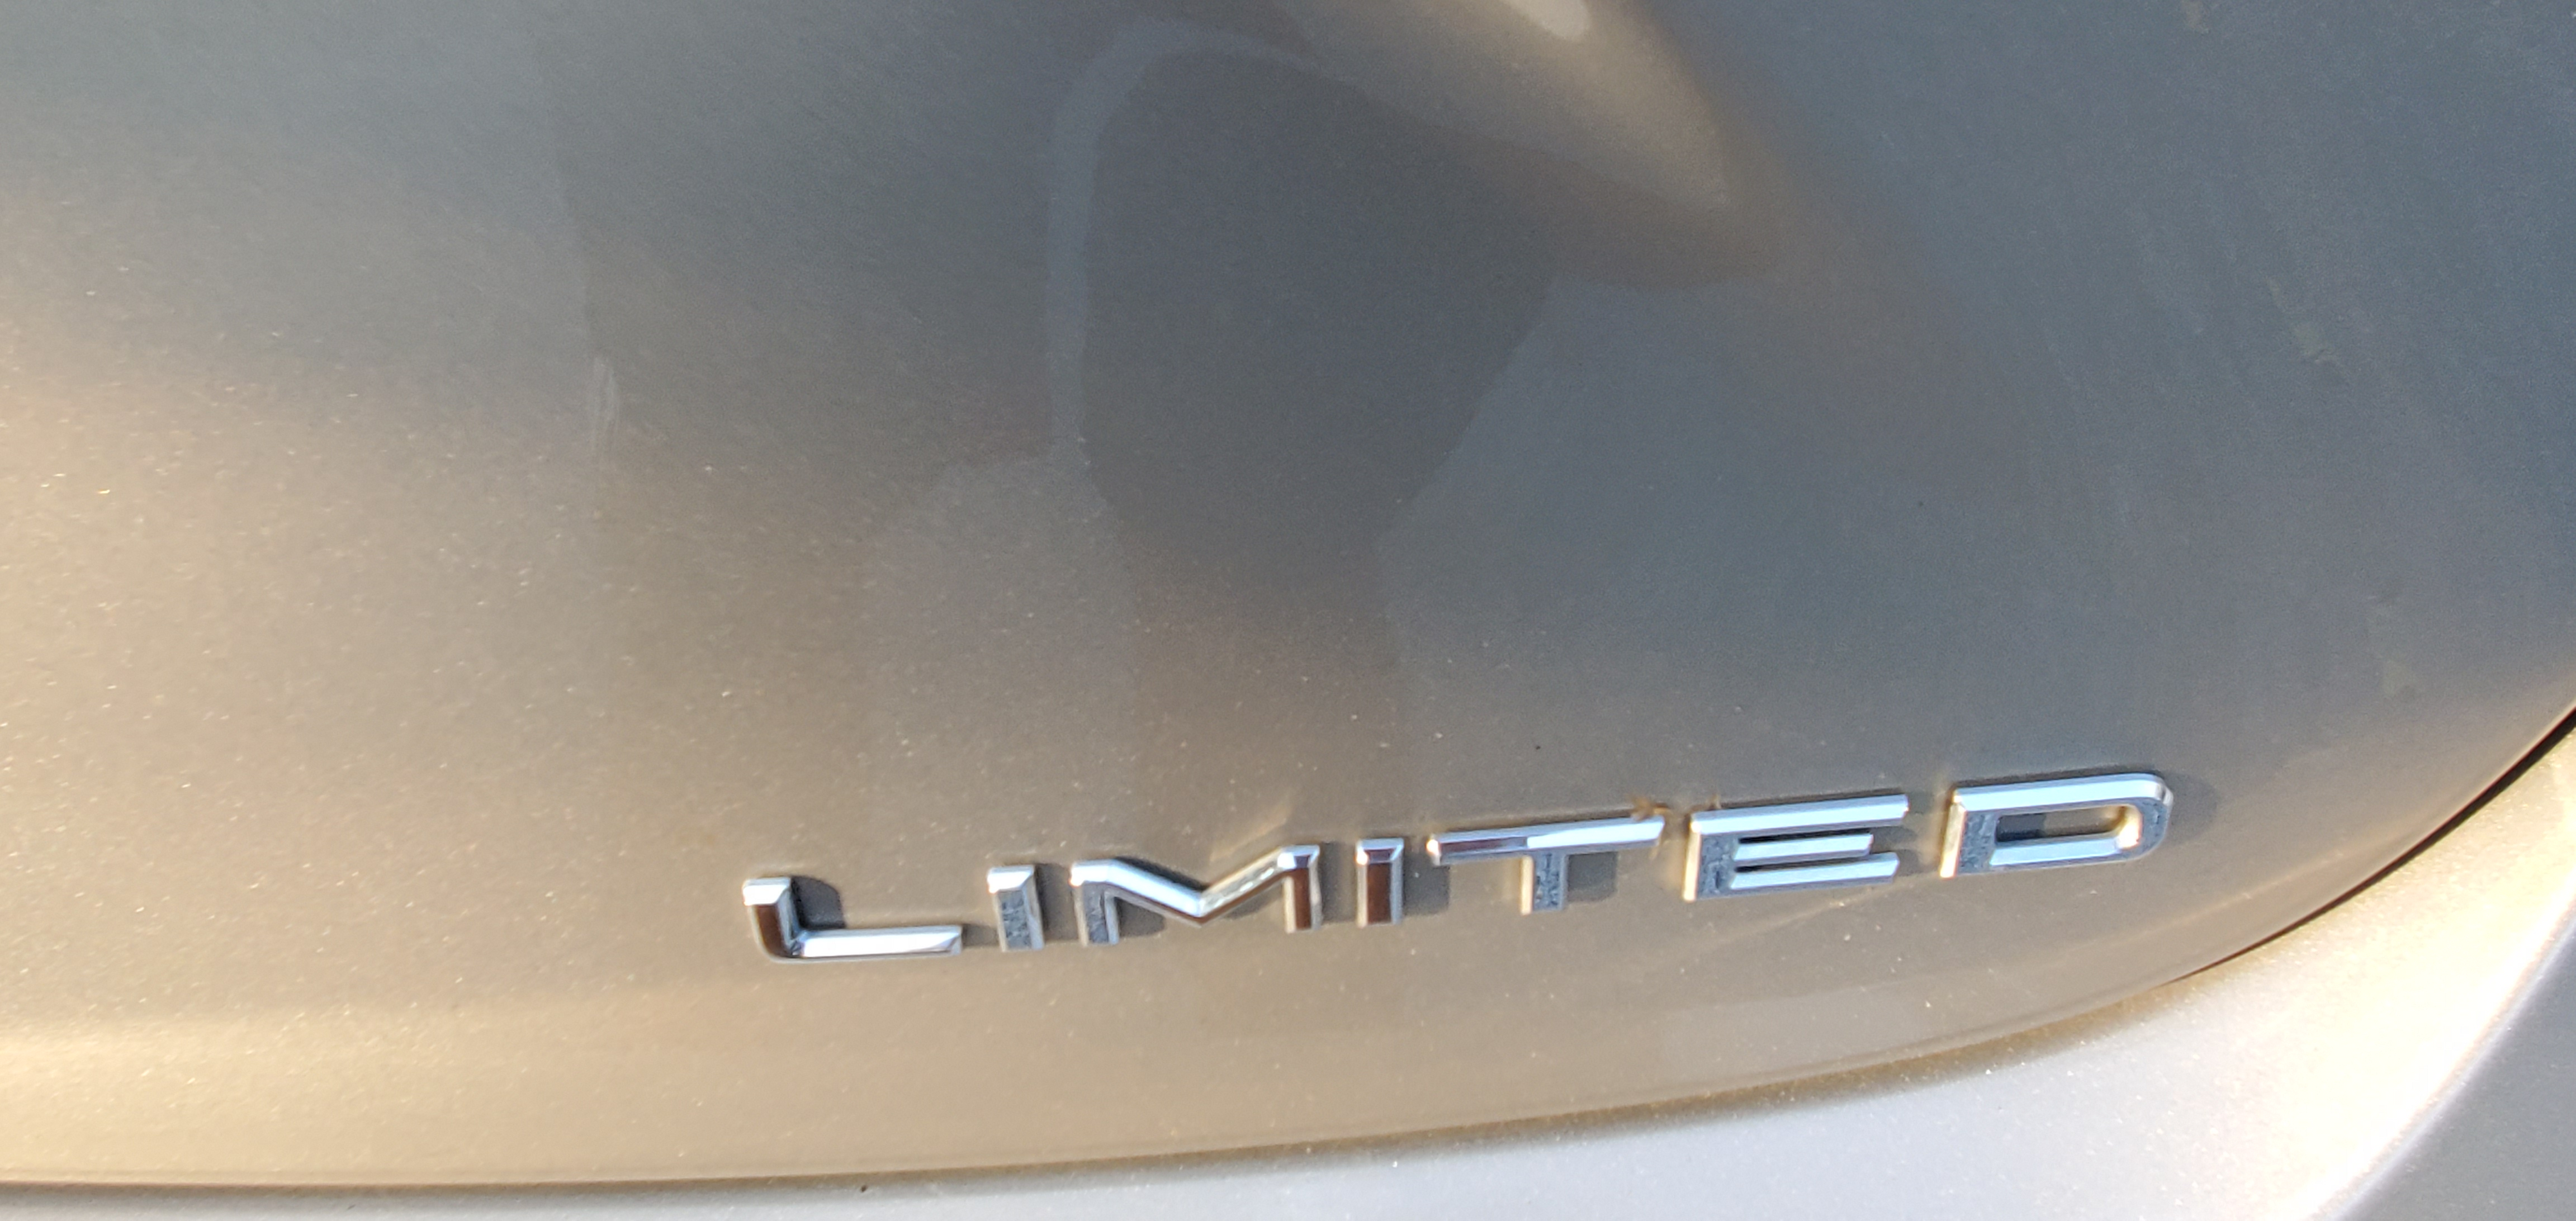
\includegraphics[width=\textwidth]{images/car_photos/20210703_192839.jpg} %8
        \caption{}
    \end{subfigure}
    \begin{subfigure}[b]{0.4\textwidth}
        \centering
        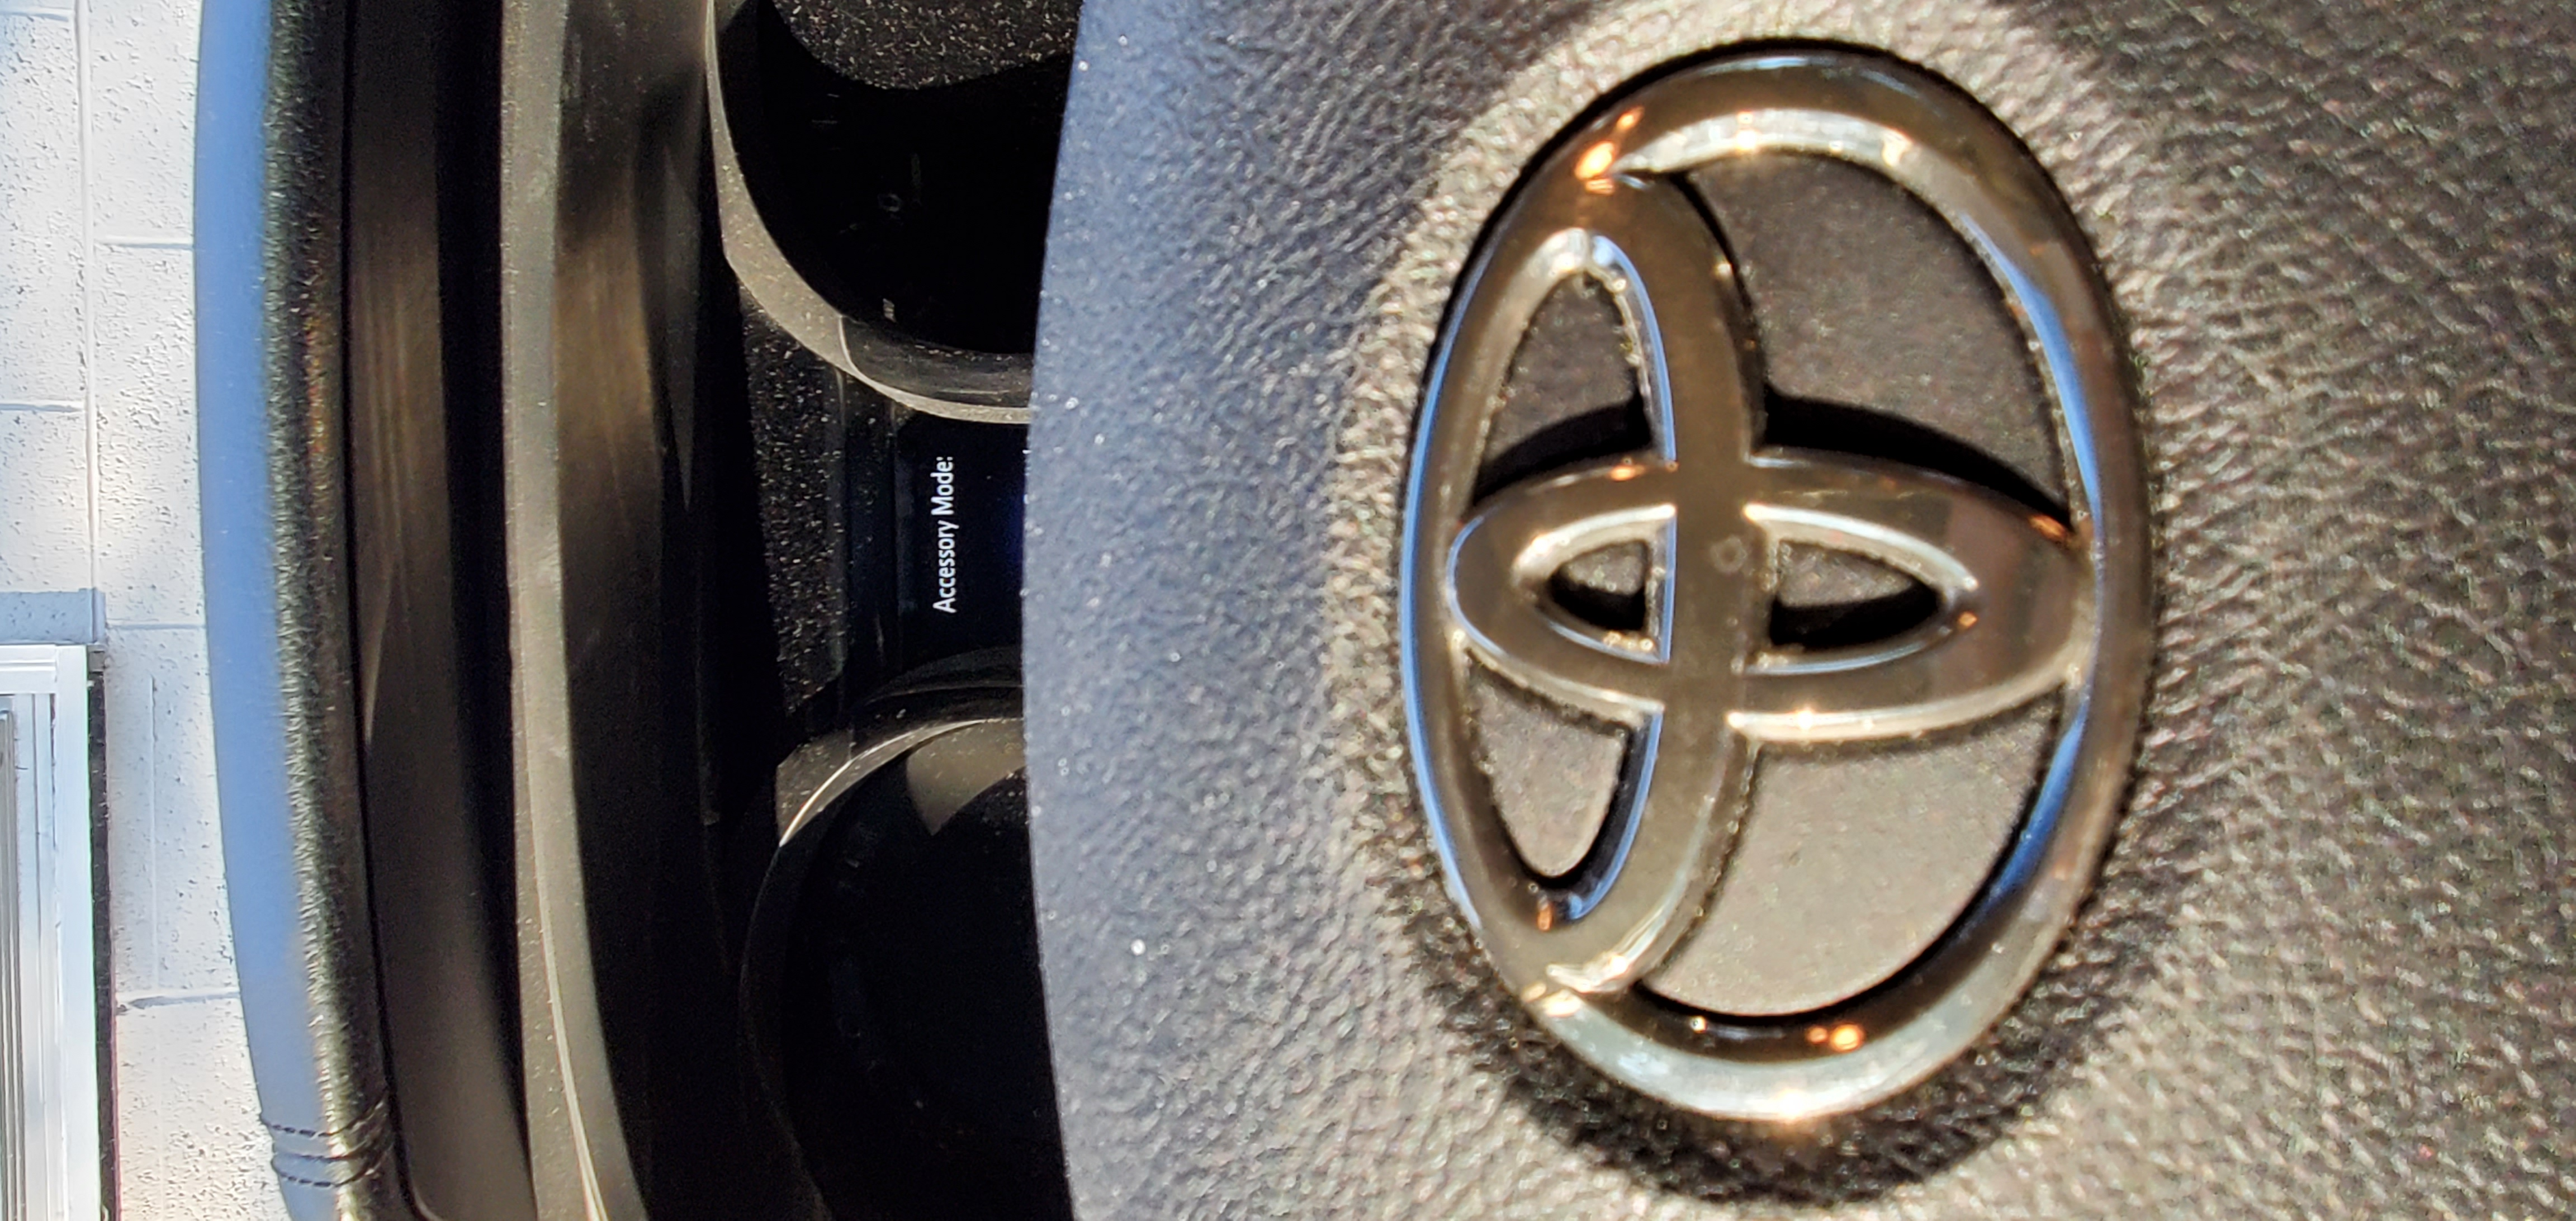
\includegraphics[width=\textwidth]{images/car_photos/20210703_192901.jpg} %9
        \caption{}
    \end{subfigure}
    \hspace{2 pt}
    \begin{subfigure}[b]{0.4\textwidth}
        \centering
        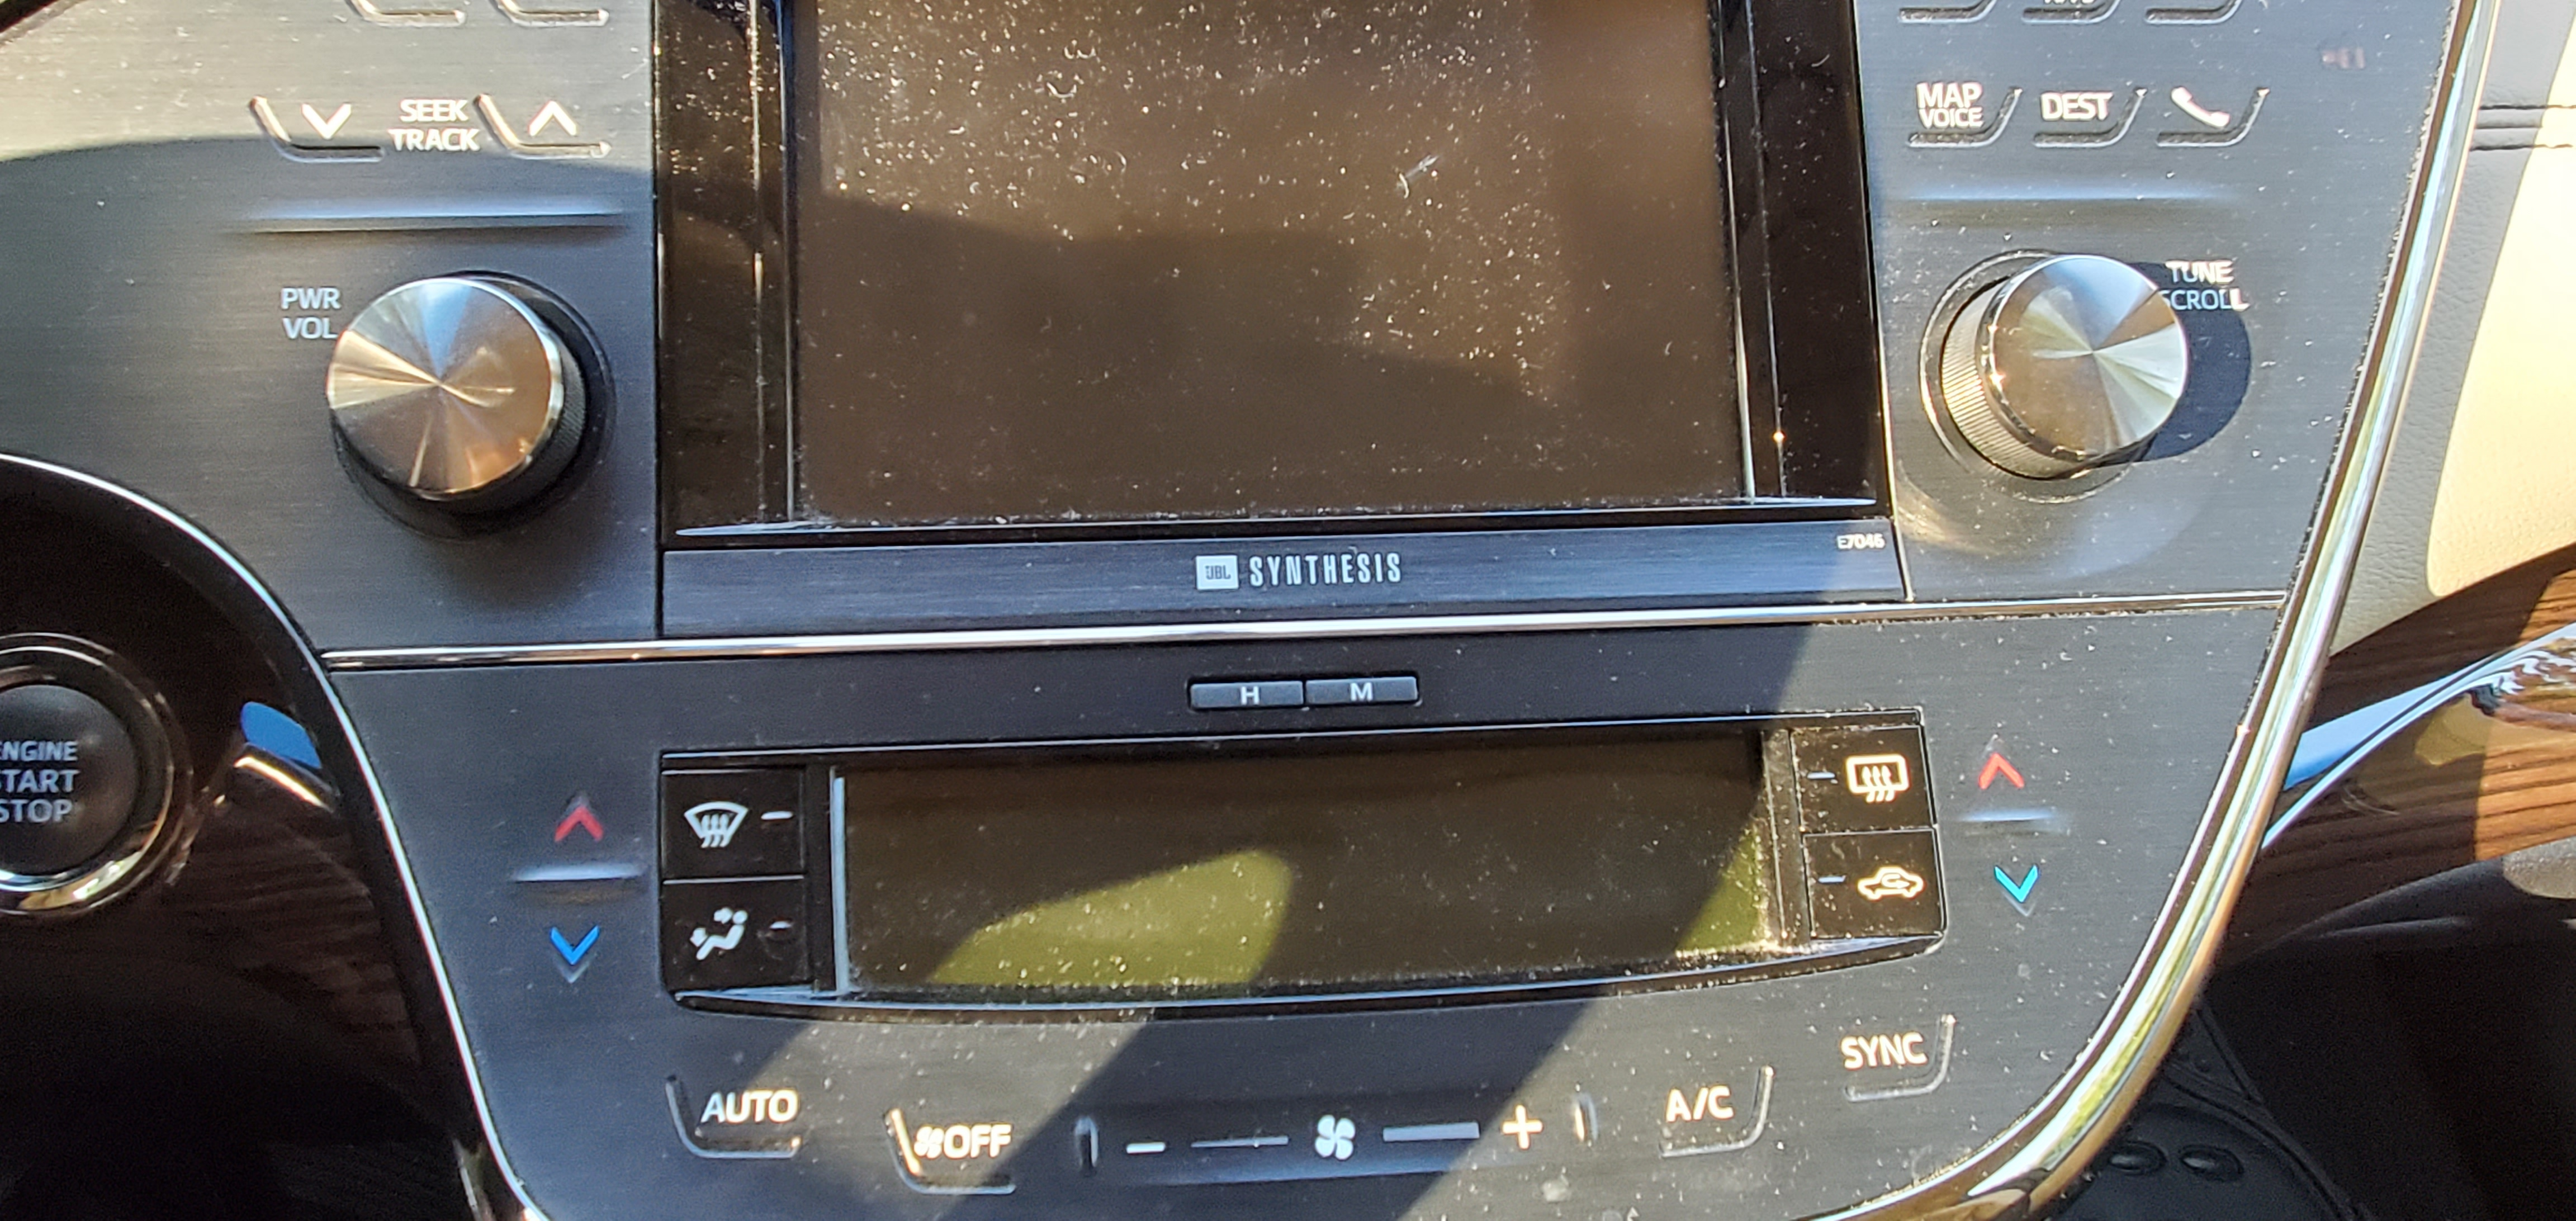
\includegraphics[width=\textwidth]{images/car_photos/20210703_192907.jpg} %10
        \caption{}
    \end{subfigure}
    \caption{Pictures of cars with capture time.}
    \label{fig:cars2}
\end{figure}

Since I didn't find any other message with other contacts, I suppose he was conducting his main business in the app Signal \cite{signal}, which is an end-to-end encrypted messaging app. I found numerous activities related to this app in the timeline.

Finally, the presence of numerous apps related to buying and selling cars, such as \textit{CarGurus} and \textit{Autotrader}, could be evidence of him selling cars on these apps.

\subsection{Recordings of the arrest}

I found a video of the arrest, which was recorded by Heisenberg, filtering the videos by date.
It was created on 20/07/2021 at 14:03:34 (UTC+0)
The MD5 hash of the video is \texttt{1fb629ceb7e03948032448b6af978c94} and the path is:\\
\texttt{Dump/data/media/0/DCIM/Camera/20210720\_150222.mp4}.

The video shows Heisenberg showing a car to a possible buyer, who is actually an undercover police officer. At the end of the video, the police officer after saying that the car is stolen, arrests Heisenberg.


\begin{figure}[!ht]
    \centering
    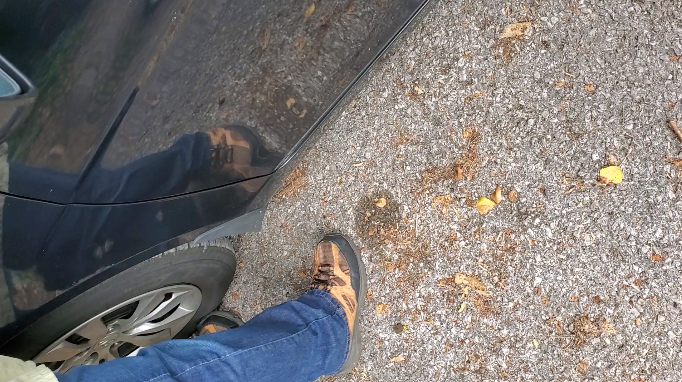
\includegraphics[width=\textwidth]{images/arrest-frame.png}
    \caption{Frame of the video showing the arrest.}
    \label{fig:rec-file}
\end{figure}

\subsection{Police best practices}

To find out if the police followed best practices, I got advantage of the timeline tool: I looked for activities on the smartphone after the arrest and I found that there are network activities in the smartphone after it. This means that the police did not follow best practices, because they should have disconnected it from the network as soon as possible and don't use it anymore. This is because the smartphone could be remotely wiped, so it is important to disconnect it from the network.

You can see for example some of the network activities during 22/07/2021 which is two days after the arrest in Figure \ref{fig:pbp}.

I retrieved the network activities in the file at the path:\\ \texttt{Dump/data/system/packages.xml}.

You can see the hash of the file in the table \ref{table:hashes}.

\begin{figure}[!ht]
    \centering
    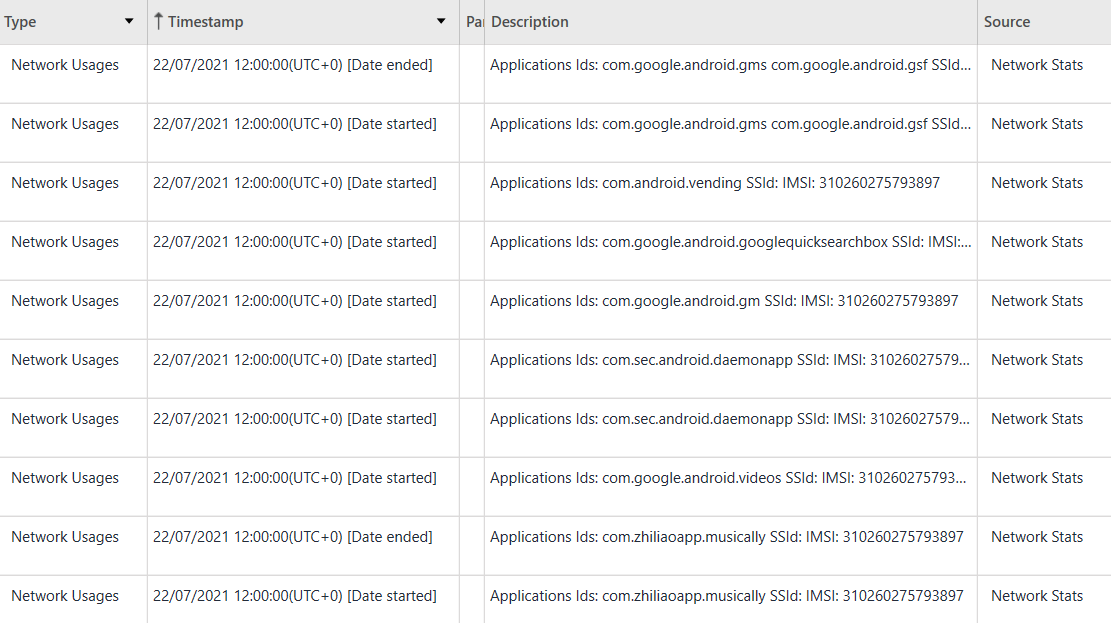
\includegraphics[width=\textwidth]{images/pbp.png}
    \caption{Network activities of the smartphone after the arrest.}
    \label{fig:pbp}
\end{figure}

\subsection{Interest in cryptocurrency}

I noticed the presence of the app \textit{Venmo} (see Figure \ref{fig:venmo-icon}), which is an app used to manage crypto wallets. I checked the timeline to see if there are any activities related to this app and I found numerous network activities related to it. You can see part of the timeline in Figure \ref{fig:crypto}.

\begin{figure}[!ht]
    \centering
    
\includegraphics[width=0.2\textwidth]{images/venmo.png}
    \caption{Icon of the app \textit{Venmo}.}
    \label{fig:venmo-icon}
\end{figure}

\begin{figure}[!ht]
    \centering
    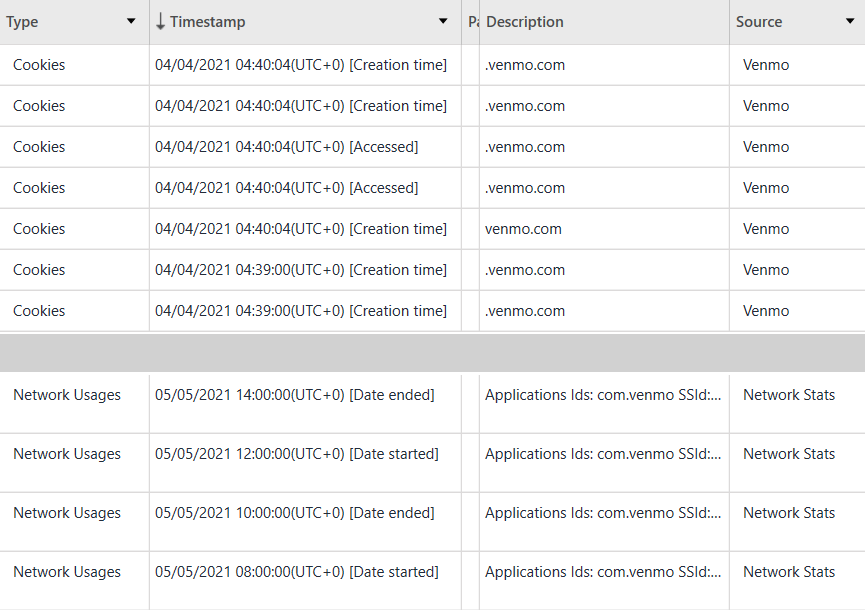
\includegraphics[width=\textwidth]{images/venmo1.png}
    \caption{Some activities of the smartphone related to the app \textit{Venmo}.}
    \label{fig:crypto}
\end{figure}

Moreover, checking Twitter notifications in Gmail, I found numerous news about cryptocurrency: he follows accounts as \textit{Bitcoin News} and \textit{Bitcoin}. See Figure \ref{fig:twitter} for some of the notifications.

\begin{figure}[!ht]
    \centering
    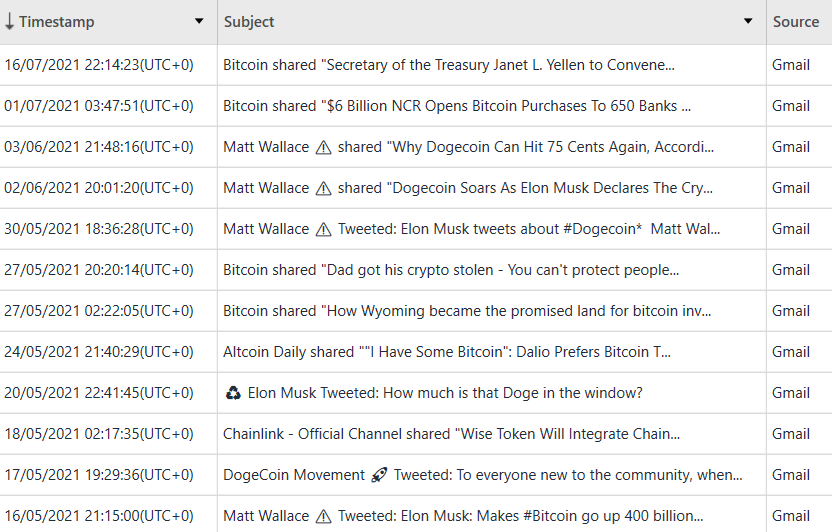
\includegraphics[width=\textwidth]{images/gmail-crypto.png}
    \caption{Some Twitter notifications about cryptocurrency.}
    \label{fig:twitter}
\end{figure}

\subsection{File hiding or encryption}
\label{sec:file-hiding}

Looking at Heisenberg's web searches I found different searches related to file hiding and encryption, such as \textit{hidden photos app}.

I found the app \textit{HideX: Calculator Lock, App Hider and Photo Vault} \cite{calculator} which is used to hide files.

The app code is \texttt{com.flatfish.calculator} and the path is the following:

\texttt{Dump/data/app/com.flatfish.calculator}. 

The app presents itself as a calculator, but it is actually used to hide files. You can see the app icon in Figure \ref{fig:calc}.

\begin{figure}[!ht]
    \centering
    
\includegraphics[width=0.2\textwidth]{images/icon.png}
    \caption{Icon of the app \textit{Calculator}.}
    \label{fig:calc}
\end{figure}

\subsection{External drives}

I found a picture in the Chrome cache related to \textit{Android USB OTG} (see Figure \ref{fig:usb}), which is a standard that allows mobile devices to connect to external drives. You can see the hash of the picture in the table \ref{table:hashes} and the path is the following:\\
\texttt{Dump/data/data/com.android.chrome/cache/Cache/ff922abbaff591ef\_0/android-\\usb-otg.jpg}.

Looking indeed at his web searches, I noticed that he searched for \textit{can a samsung micro usb connector transfer data} and \textit{how to mount a pendrive on android} (see Figure \ref{fig:web}).

Given these information, I suppose that he wanted to connect a pendrive to his smartphone to transfer data.

\begin{figure}[!ht]
    \centering
    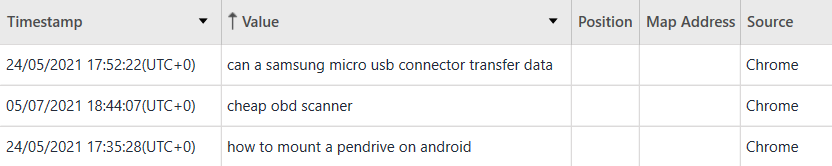
\includegraphics[width=\textwidth]{images/web-searches.png}
    \caption{Web searches concerning external drives.}
    \label{fig:web}
\end{figure}

\begin{figure}
    \centering
    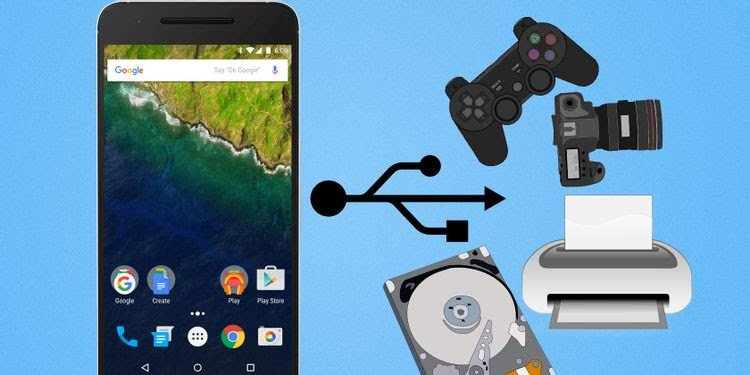
\includegraphics[width=0.5\textwidth]{images/android-usb-otg.jpg}
    \caption{Picture found in the cache of Chrome.}
    \label{fig:usb}
\end{figure}

\subsection{Hidden image}

Thanks to the search bar, I found the image with the following MD5 hash: \\
\texttt{066858f4b1971b0501b9a06296936a34}. 

The path is \texttt{Dump/data/data/com.flatfish.cal.privacy/cache/image\_manager\_disk \\ \_cache/7ae6e97ba4ad0d693413273d6e270a412af3331a9c96c7a9049e3ae9b6047c9d.0}.

We can see that the picture was hidden with the app \textit{HideX: Calculator Lock, App Hider and Photo Vault} (see Section \ref{sec:file-hiding}): I found it in the cache of the app (see Figure \ref{fig:cache}).

\begin{figure}[!ht]
    \centering
    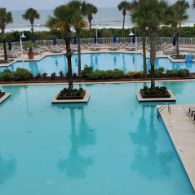
\includegraphics[width=0.5\textwidth]{images/hidden.png}
    \caption{Hidden image.}
    \label{fig:cache}
\end{figure}

\subsection{Meeting with \texttt{+15402993169}}

I found the messages exchanged with \texttt{+15402993169}: you can see part of the messages in Figure \ref{fig:meeting}, where the meeting is arranged. They planned to meet on 20/07/2021 at 19:00 at the Washington Street Tennis Court.

\subsection{Signal app usage}

To check the last usages of the app Signal \cite{signal} on 14/07/2021, I used the timeline tool, given that the app code is \texttt{org.thoughtcrime.securesms}.
You can see part of the timeline in Figure \ref{fig:signal}.

The last usage of the app on 14/07/2021 was at 20:00:00 (UTC+0).

\begin{figure}[!ht]
    \centering
    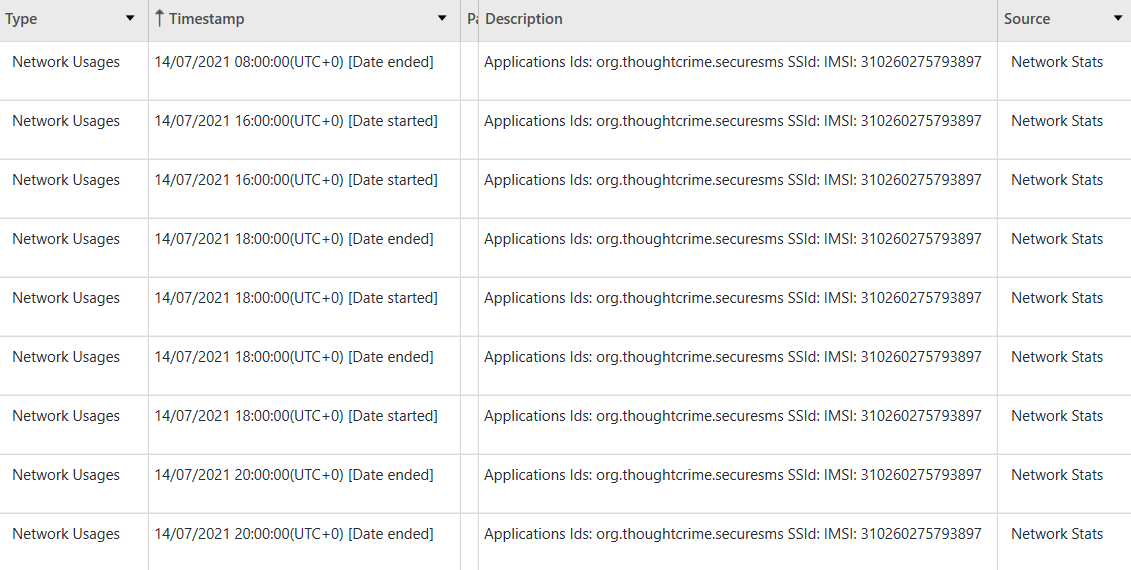
\includegraphics[width=\textwidth]{images/signal.png}
    \caption{Activities of the smartphone related to the app \textit{Signal}.}
    \label{fig:signal}
\end{figure}

\addcontentsline{toc}{chapter}{References}
\printbibliography[title={References}]

\end{document}